%%%% body
\begin{abstract}
  In this paper, we consider the problem of transforming the Suffix Array ($\SA$) of a string $S$ of length $n$ into its Compact Directed Acyclic Word Graph (CDAWG) $G$.
  %% We aim to achieve this transformation using time and working space bounds sensitive to the size of $G$, the numbers of maximal repeats, right- and left-extensions, denoted by $\mu(S)$, $e_R(S)$ and $e_L(S)$, respectively.
  This work extends the classic problem of transforming the Suffix Array of $S$ into its suffix tree in the context of output-sensitive computation on repetition-aware text indexes
  Our main result is a simple and efficient algorithm that solves this problem in
  $O(e_R(S) + e_L(S))$ time and
  %% $O(e_R(S) + e_L(S) + \mu(S)\log \mu(S))$ time and
  $O(e_R(S) + e_L(S))$ space.
  This requires $O(e_R(S) + e_L(S))$ probes to an index structure $\sig I$ consisting of the $\SA$ and $\ISA$ arrays,
  and a Range Minimum Query (RMQ) structure on and $\LCP$ array
  (of $O(n)$ size).
  %% and $\LCP$ arrays (of $O(n)$ size), where the $\LCP$ array is augmented with a Range Minimum Query (RMQ) structure.
As an application, we demonstrate that this leads to an $O(e\cdot\polylog(n))$ time and space algorithm for constructing the CDAWG of S directly from the \textit{r-index}, proposed by Gagie, Navarro, and Prezza (J.~ACM, 67:1, 2020), which has a size of $O(r\cdot\polylog(n))$.
To achieve the above results, we devise two novel methods that may be of independent interest:
(ii) A method for enumerating all maximal repeats in $O(e_R(S) + e_L(S))$ time, requiring only $O(\sigma \log n)$ auxiliary working space in addition to the space of $\sig I$. 
(ii) A method for computing the suffix links from the CDAWG of S without suffix links (or its $\LPT$-tree, the extended longest prefix tree) in $O(e_R(S) + e_L(S))$ time and space.
\end{abstract}


%% \begin{abstract}
%% In this paper, we consider the problem of transforming the Suffix Array ($\SA$) of a string $S$ of length $n$ into its Compact Directed Acyclic Word Graph (CDAWG) $G$. We aim to achieve this transformation using time and working space bounds sensitive to the size of $G$, the numbers of maximal repeats, right- and left-extensions, denoted by $\mu(S)$, $e_R(S)$ and $e_L(S)$, respectively. This work extends the classic problem of constructing a suffix tree from a Suffix Array within the context of repetition-aware text indexes.
%% Our main result is a simple and efficient algorithm that solves this problem in $O(e_R(S) + e_L(S) + \mu(S)\log \mu(S))$ time and
%% $O(e_R(S) + e_L(S))$ space. This requires $O(e_R(S) + e_L(S))$ probes to an index structure $\sig I$ consisting of the $\SA$, $\ISA$, and $\LCP$ arrays (of $O(n)$ size), where the $\LCP$ array is augmented with a Range Minimum Query (RMQ) structure.
%% As an application, we demonstrate that this leads to an $O(e\cdot\polylog(n))$ time and space algorithm for constructing the CDAWG of S directly from the \textit{r-index}, proposed by Gagie, Navarro, and Prezza (J.~ACM, 67:1, 2020), which has a size of $O(r\cdot\polylog(n))$.
%% To achieve the above results, we devise two novel methods that may be of independent interest:
%% (ii) A method for enumerating all maximal repeats in $O(e_R(S) + e_L(S))$ time, requiring only $O(\sigma \log n)$ auxiliary working space in addition to the space of $\sig I$. 
%% (ii) A method for computing the suffix links from the CDAWG of S without suffix links (or its $\LPT$-tree, the extended longest prefix tree) in $O(e_R(S) + e_L(S))$ time and space.
%% \end{abstract}





%%%%% body %%%%%%%%%%%%%%%%%%%%%%%%

%%%% 
\section{Introduction}
\label{sec:intro}

\subsection{Background}
%% \mysubsubsection{Background}
%%% 
The goal of the problem is to transform the suffix array of a string $S$ (Manber and Myers~\cite{manber:myers1993suffixarrays}) with length $n$ into an equivalent DAG-based string index structure, called the \textit{CDAWG} (\textit{Compact Directed Acyclic Word Graph}), of the string (Blumer, Blumer, Haussler, McConnell, and Ehrenfeucht~\cite{blumer1987complete}). Here, the CDAWG of a string $S$ is the path-compacted smallest automaton $C$ for accepting the set of all suffixes of $S$.
Although both structures, given a string $S$ of length $n$, compactly%
%%%%
\myfootnote{In recent literature, an index structure for a string is commonly called compact if it stores a string S of length n using $O(n \log\sigma)$ bits, where $\sigma$ is the size of the underlying alphabet. However, throughout this article, we use the term compact in the context of graph-based indexes, such as suffix trees or DAWGs. A structure is defined as \textit{compact} if it employs path-compression to represent all $O(n^2)$ possible factors of $S$ in $O(n)$ or fewer words (see, e.g., Crochemore, Hancart, and Lecroq~\cite{crochemore2007algorithms:on:strings}).  
}
%%%%
store all of $O(n^2)$ factors in linear or less words of space supporting a similar set of operations efficiently, the latter compresses the former by reducing its space from $O(n)$ to $O({e_R(S) + e_L(S)})$, where $e_R(S)$ and $e_L(S)$ are parameters that measure the compressibility of a string, defined as the numbers of all right- and left-extensions of maximal repeats of $S$, respectively.
Belazzougui \textit{et al.}~\cite{belazzougui:nunial:gagie:prezza:raffinot2015composite} showed that both of $e_R(S)$ and $e_L(S)$ upperbounds the size $z(S)$ of the LZ-parse and the number $r(S)$ of runs of BWT of $S$.

%% where ${e_R(S) + e_L(S)}$ is a parameter that measures the compressibility of a string. The parameter ${e_R(S) + e_L(S)}$ is defined as the sum of the the numbers $e_R$ and $e_L$ of all right- and left-extensions of the maximal repeats of the string.

%%%%%%
\begin{figure}[t]
\begin{minipage}[c]{0.44\textwidth}
\centering
\raisebox{-.5cm}{ %height
\nofbox{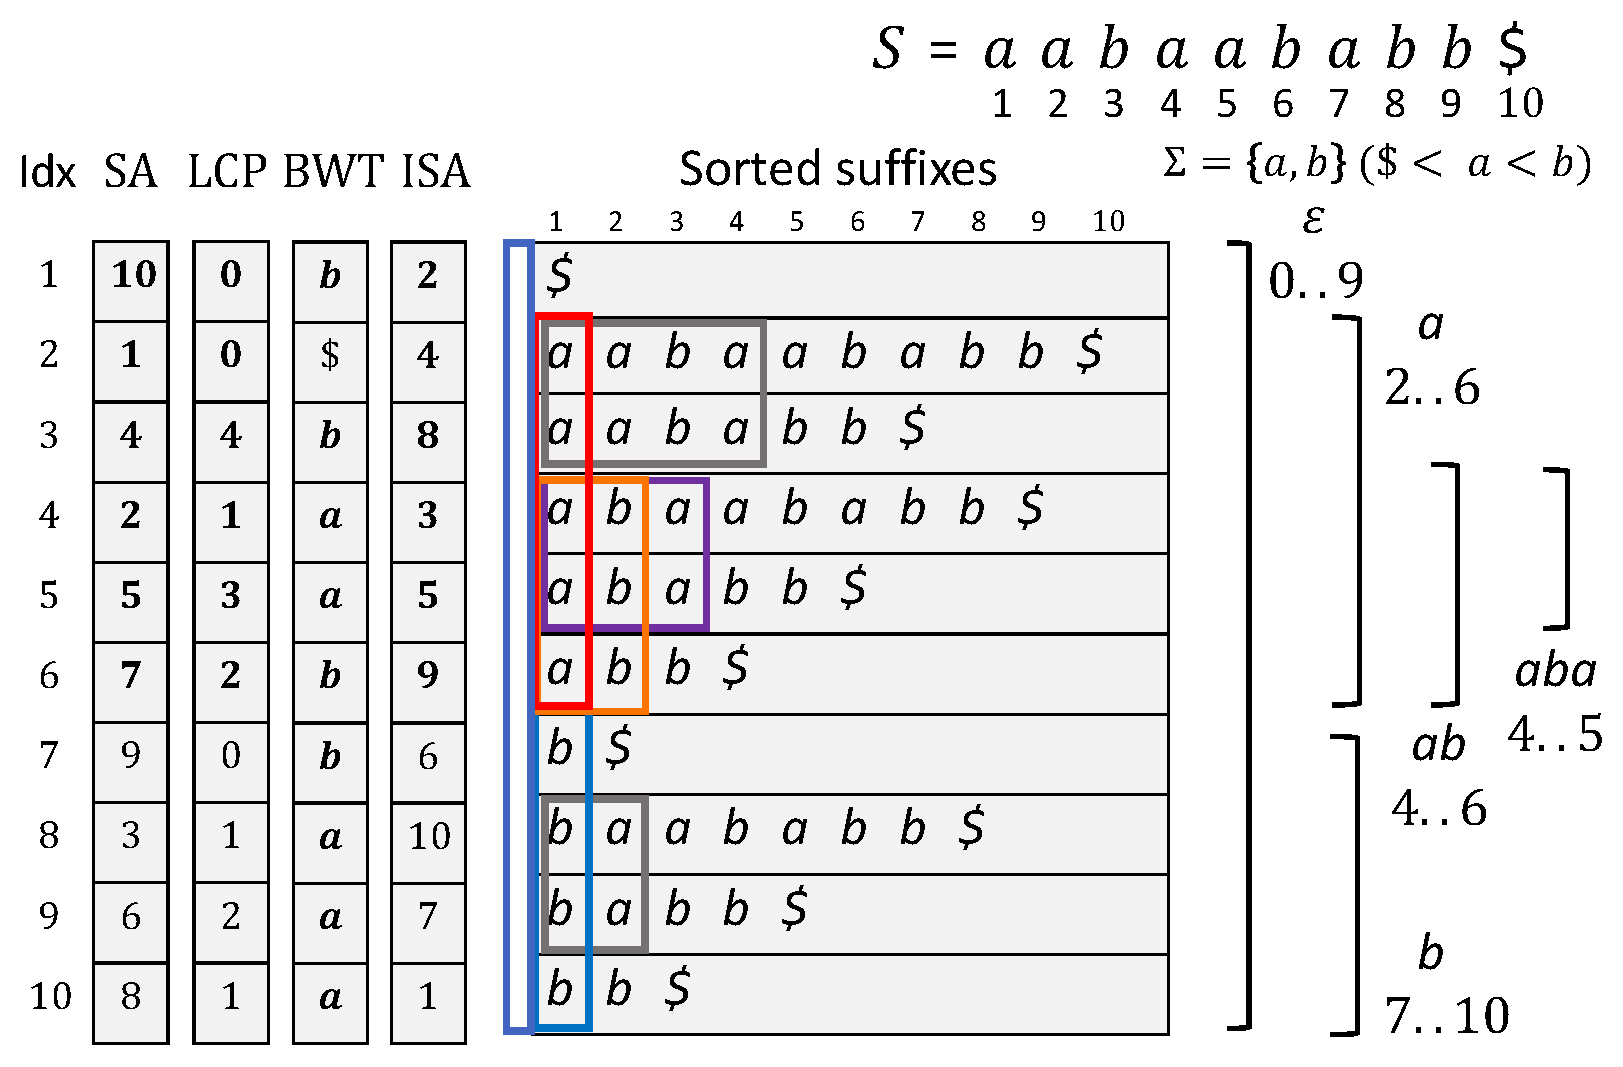
\includegraphics[height=.90\textwidth]{fig1.pdf}}
}
\end{minipage}
\hspace{20mm}
\begin{minipage}[c]{0.44\textwidth}
\centering
\nofbox{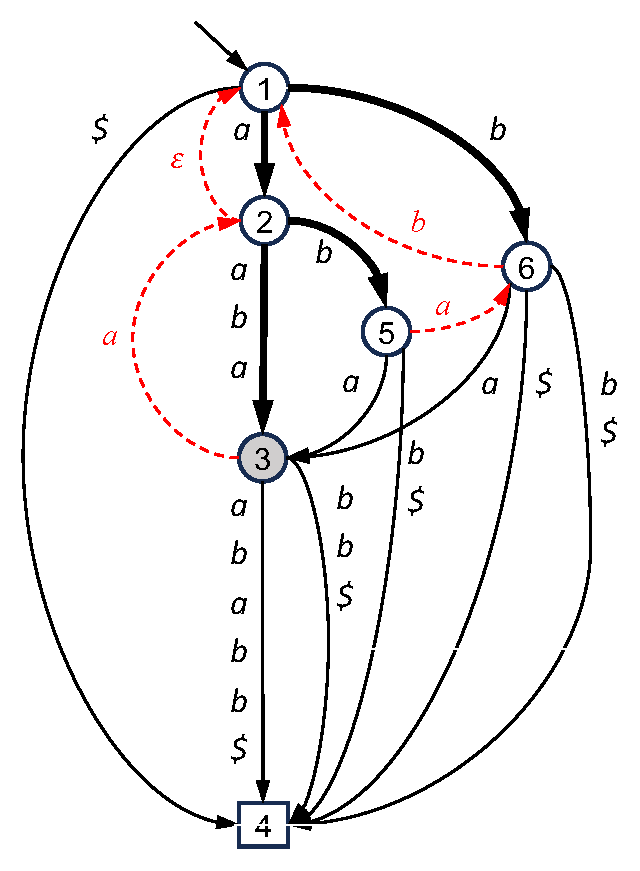
\includegraphics[height=.95\textwidth]{fig2a.pdf}}
\end{minipage}
%% \vspace{.5\baselineskip}
\caption{An Example of an input and an output of the transformation problem with a string $S[1..10] = aabaababb\daller$ of length $n = 10$ over an alphabet $\Sigma = \set{a, b, \daller}$ (top).
  An input is the index $\sig I$ of arrays $SA, LCP, BWT, ISA$ and $S$ (left). An output is the CDAWG $G$ of $S$ (right).
  In $G$, black thick, black thin, and red dashed arrows, respectively, indicate solid and non-solid edges, and suffix links.
  A range with a string correspond to a node of $G$ and its representative. 
  %% We observe that branching nodes $1, 3,14,12$, and $6$ of $G$ correspond to maximal repeats of $S$, namely, $\eps$, $a$, $b$, $ab$, and $aaba$. 
}\label{fig:example:problem}
\end{figure}
%%%%%%


\subsection{Problem}
%%% 
In this paper, 
%article,
we study the following question. 

\vspace{-0.25\baselineskip}
\begin{trivlist}{\item[] \noindent \textbf{Question.}
How to build the CDAWG $G$ of a string $S$ from the suffix array with auxiliary arrays and structures of total length $O(n)$ in output-sensitive time and space, that is, in the time and working space proportional to the output size ${e_R(S) + e_L(S)}$ of $G$?
}\end{trivlist}
\vspace{-0.25\baselineskip}


As read-only inputs, we assume an index structure $\sig I$ consisting of the following structures (Manber and Myers~\cite{manber:myers1993suffixarrays}) preprocessed from $S$ beforehand: 
\begin{itemize}
\item the suffix array $\SA$,
\item the inverse suffix array $\ISA$,
\item the longest common prefix array $\LCP$ augmented by the range-minima query (RMQ) structure (denoted by $\LCP_{RMQ}$).%
\footnote{
The \textit{RMQ query on LCP} asks, given any ssubrange $i..j \subseteq 1..n$, to return the minimum of the LCP-values $\set{LCP[k] \mid 1\le k\le j}$ within $i..j$.
}
\end{itemize}

All of the above structures occupy $O(n)$ words of space, and can be constructed in $O(n)$ time from a string $S$ over an integer alphabet in preprocessing (for details, see the textbook or survey article by Navarro~\cite{navarro2016cds:book,navarro2021indexing:ii}).
\cref{fig:example:problem} shows an example of input and output of the problem.

An intended application scenario for the above problem, such as in bioinformatics databases or text repositories, is as follows: the structure $\sig I$ is constructed once, resides in memory using $O(n)$ space, and will be used repeatedly for tasks including CDAWG generation and string searching spending $o(n)$ time. 

%% n intended application senario of the above question, e.g., in bioinformatics databases or text repositories, is as follows: the structure $\sig I$ is constructed once, resides on memory using $O(n)$ space, and will be used many times for CDAWG generation, and other tasks such as the string search.

%Finally, we introduce a class of the repetitiveness measures for a string $S$ according to Belazzougui \textit{et al.}~\cite{belazzougui:nunial:gagie:prezza:raffinot2015composite}. $\mu(S)$, $e_R(S)$, and $e_L(S)$ are the numbers of all maximal repeats, all right- and all left-extensions of maximal repeats, respectively.


%% Belazzougui \textit{et al.}~\cite{belazzougui:nunial:gagie:prezza:raffinot2015composite} showed that the parameter $e_R(S)$ upperbounds popular compression parameters $z(S)$ and $r(S)$ from above, that is, $\max\{z(S), r(S)\} \le e_R$, where $z(S)$ and $r(S)$ are the numbers of \textit{phrases of the Lemple-Ziv parse} of $S$ and \textit{equi-letter runs of the Burrows-Wheeler transform} of a string~$S$. 
%% We remark that these parameters $e_R(S)$ and $e_L(S)$ can be $\Theta(n)$ in the worst case, while they can be logarithmically smaller than $n = |S|$ for some classes of strings, e.g., Fibonacci and Thue-Morse words.



\subsection{Results}
%%% 
Under the problem setting above, we show the main results of this paper. 

\begin{theorem}[main result]\label{thm:main:index:cdawg}
  Let $S$ be any string of length $n$ over an integer alphabet $\Sigma$ of size $\sigma \ge 2$, and
  $\sig I = (\SA, \ISA, \LCP_{RMQ})$ be the afoementioned index structure of $O(n)$ total size. 
  There exists an algorithm that can transform $\sig I$ and
  $S$ into the CDAWG of $S$
  in $O(e_R(S) + e_L(S))$ time
  %% in $O(e_R(S) + e_L(S) + \mu(S)\log\mu(S))$ time
  and 
  $O(O(e_R(S) + e_L(S))$ words of working space,
  %% $O(\max\{O(e_R(S) + e_L(S), \sigma\log n\})$ working space,
  %% where the algorithm probes
  probing at most $O(e_R(S) + e_L(S))$ cells of $\sig I$ and $S$. 
\end{theorem}

From \cref{thm:main:index:cdawg} above, the proposed algorithm improves the time and space complexity $\Theta(n)$ of the straightforward algorithms via suffix tree construction~\cite{raffinot2001maximal} to asymptotic time and space complexity $O(e_R(S)+e_L(S)$ for classes of repetitive texts with $\max\set{e_R(S), e_L(S)} = o(n)$.
%%
%% Since it solves computaton of the set $\MR(S)$ of all distinct maximal repeats of $S$, we have the next corollary.
On enumeration of the set $\MR(S)$ of all distinct maximal repeats of $S$, we have the next result. 


\begin{theorem}\label{cor:main:index:maxrep}
  Under the same assumption to \cref{thm:main:index:cdawg}, 
  the set $\MR(S)$ of all distinct maximal repeats of a string $S$ can be enumerated in $O(e_R(S)+e_L(S))$ time and $O(\sigma \log n)$ working space using $O(e_R(S) + e_L(S))$ probes to $\sig I$ and $S$, where $n = |S|$ is the length of $S$. 
\end{theorem}

\mysubsubsection{Application to compressed text indexes}
%%%
Recently, repetition-aware indexes have attracted much attention. A recent compressed index, called \textit{r-index}, proposed by Gagie, Navarro, and Prezza~\cite{gagie:navarro:prezza2020fully} as well as a variant by Nishimoto and Tabei~\cite{nishimoto2022optimaltime:rlbwt:construction} occuppy $O(r(S)\polylog(n))$ space and covers the functionality of the afoementioned index $\sig I$ and $S$. In this setting, we have the next theorem from \cref{thm:main:index:cdawg}. 


\begin{theorem}[compressed computation]\label{thm:rindex:all}
  Let $S$ be any string of length $n$ over an integer alphabet $\Sigma$ of size $\sigma \ge 2$. There exist algorithms that solve each of the problems below in $O((e_R(S) + e_L(S))\cdot \polylog(n))$ time and 
  $O(e_R(S) + e_L(S))$ words of working space,
  based on the r-index $\sig R$  of $O(r(S)\cdot\polylog(n))$ space
  by probing $O(e_R(S) + e_L(S))$ cells of $\sig R$ and $S$: 
\begin{enumerate*}[(1)]
\item Construction of the CDAWG of $S$; 
\item Enumeration of all distinct maximal repeats in $\MR(S)$,  
\end{enumerate*}
\end{theorem}

%% \begin{theorem}\label{thm:compressed:index:cdawg}
%% There exists an algorithm that can transform the r-index $\sig R$ of a string $S$ of length $n$ over an integer alphabet into the CDAWG $G$ of $S$
%%   in $O((e_R(S) + e_L(S))\cdot \polylog(n))$ time
%%   using $O(r(S)\cdot \polylog(n) + O(e_R(S) + e_L(S))$ working space,
%%   where the algorithm probes at most $O(e_R(S) + e_L(S))$ cells of the r-index $\sig R$ of $O(r(S)\cdot\polylog(n))$ size. 
%% \end{theorem}


%% By applying \cref{thm:compressed:index:cdawg} to enumeration of maximal repeats based on the r-index of a string, we have the next corollary. 

%% \begin{corollary}[maximal repeats enumeration on the r-index]\label{cor:main:index:maxrep}
%%   There exists an algorithm that can enumerate the set $\MR(S)$ of all distinct maximal repeats of a string $S$ in 
%%   $O((e_R(S)+e_L(S))\cdot \polylog(n))$ time 
%%   and $O(\sigma \log n)$ working space,
%%   by probing  $O(e_R(S) + e_L(S))$ cells of the r-index $\sig R$ of $S$.
%%   %%with $O(r(S)\cdot\polylog(n))$ size. 
%% \end{corollary}


From the corollary, our method can be an alternative to the repetition-aware algorithm (namely, the r-enum) for distinct maximal repeats by Nishimoto and Tabei~\cite{nishimoto:cpm2021enum}.
%% It is also time efficient than approaches of using as a base algorithm the traversal algorithm by Abouelhoda \textit{et al.}~\cite{abouelhoda2004replacing} or one by Narisawa \textit{et al.}~\cite{narisawa2007efficient}. 


%%Fibonacci and Thue-Morse words.
%% Since it is known that both of ${e_R(S) + e_L(S)}(S)$ and $r$ are $\Theta(\log n)$ for any Thue-Morse words of length $n$,

%%%%%%
\begin{figure}[t]
\centering
\begin{minipage}[c]{0.42\textwidth}
\centering
\nofbox{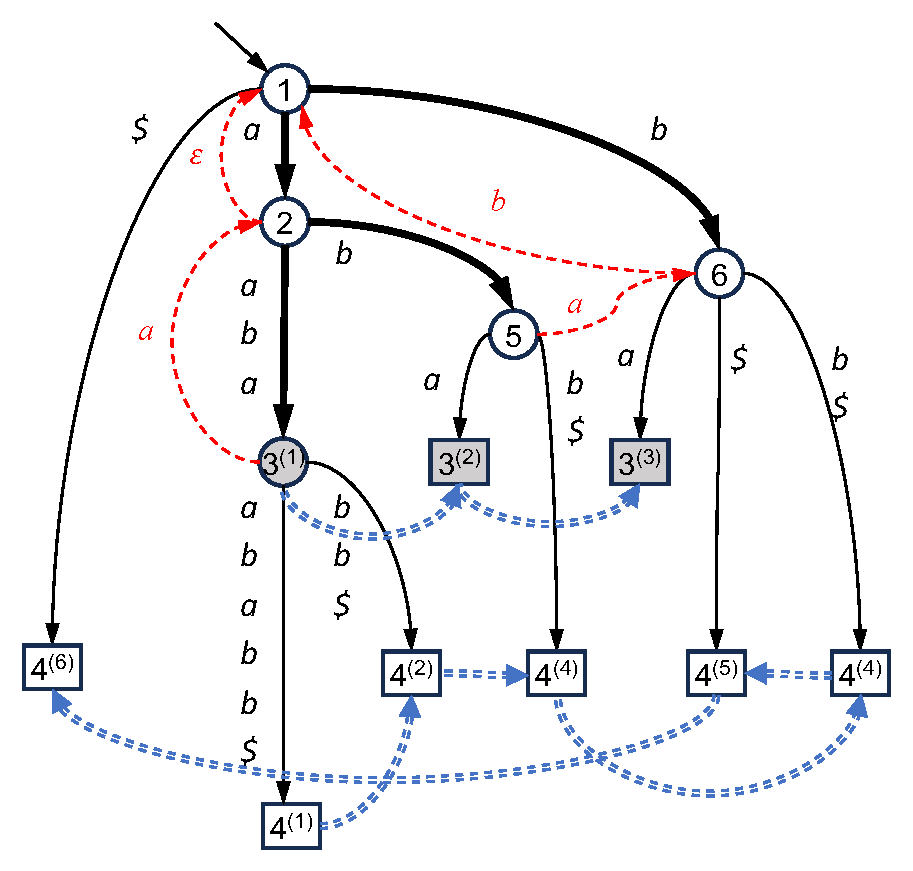
\includegraphics[height=1.0\textwidth]{fig2b.pdf}}
\end{minipage}
%% \vspace{.5\baselineskip}
\caption{An example of an intemediate structure, called the \LPTrm-tree, $T$ of a string $S = aabaababb\daller$ in \cref{fig:example:problem}.
Circles and boxes indicate branching nodes and leaves. Black thick, black thin, and red dashed arrows, respectively, indicate solid and non-solid edges, and suffix links.
  A collection of nodes connected by double dotted arrows indicates a congruence class w.r.t.~the end-positions, which will be merged into a node in the CDAWG. 
  %% Sets of nodes connected by double dotted arrows, namely, $\set{3\rk 1, 3\rk 2, 3\rk 3}$ and $\set{4\rk 1, \dots, 4\rk 6}$ form a congruence class of $\eqepos$ w.r.t.~end-positions, and is merged into a node in the CDAWG of $S$. 
}\label{fig:example:lpttree}
\end{figure}
%%%%%%

\mysubsection{Related work}
%%%
It is well-known (see, e.g., ~\cite{crochemore2021book125problems:chap:satostree}) that the problem of transforming the suffix array (SA) of a string $S$ into its suffix tree $T$ can be solved in $O(n)$ time and space using the LCP array with auxiliary stack, which is done by simulation of traversal of the suffix tree based on either the bottom-up traversal of by Kasai \textit{et al.}~\cite{kasai:lee2001lcp:linear},
or the top-down traversal by Abouelhoda \textit{et al.}~\cite{abouelhoda2004replacing}.
%%
For the closely related problem of enumerating the set $\MR(S)$ of all maximal repeats of a string $S$, recent algorithms for enumerating $\MR(S)$ in $O(n)$ time, $O(n)$-space algorithm by Beller \textit{et al.}~\cite{beller:berger2012space:efficient:bbo} and $O(r\polylog(n))$-space algorithm by Nishimoto and Tabei~\cite{nishimoto:cpm2021enum}, simulate the top-down traversal of the \textit{Weiner tree} of $S$ --- the rooted tree formed by the reversed suffix links ---  based on BWT of $S$ augmented with the \textit{Wavelet tree}~\cite{grossi2003high}.

Recently, Cleary and Dood~\cite{cleary2023constructing} proposed an algorithm for constructing the CDAWG of a string in the form of a grammar using the LCP-intervals of maximal repeats of the string. However, they did not propose any algorithm to compute such LCP-intervals in $O(e_R(S) + e_L(S))$ time and space.

The relationship between the size of the CDAWG and the parameter ${e_R(S) + e_L(S)}$ was first studied by Raffinot~\cite{raffinot2001maximal}, and the use of ${e_R(S) + e_L(S)}$ as a compression parameter was proposed by Belazzougui \textit{et al.}~\cite{belazzougui:nunial:gagie:prezza:raffinot2015composite}.

\mysubsubsection{Organization of this paper}
\cref{sec:prelim} introducing some definitions and notation. 
\cref{sec:sa:to:lpt} first presents how to transform the suffix array of a string $S$ to its \LPTrm-tree in $O(e_R + e_L\log n)$ time, and  
\cref{sec:lpt:to:cdawg} presents how to transform the \LPTrm-tree into the final CDAWG of $S$. Combining these results, \cref{sec:analysis} shows a final algorithm for converting the suffix array of $S$ into its CDAWG. 
Finally, \cref{sec:concl} show conclusion and future work.

%%%%
\section{Preliminaries}
\label{sec:prelim}

We introduce necessary definitions and notation in this paper according to~\cite{charalampopoulos2018extended,barton2014linear,ilie2011minimum,belazzougui2020linear}. 
%% \mysubsubsection{Basic definitions}
For any integers $i\le j$, we denote by $i..j$
%or $[i..j]$
the interval $\set{i, i+1, \dots, j}$. For a set $A$, we denote by $|A|$ the \textit{cardinality} of $A$, by $A^*$ and $A^+$ the \textit{sets of all finite sequences} of lengths $\ge 0$ and $\ge 1$ over $A$, respectively.
%%% 
As a model of computation, we assume the \textit{unit-cost RAM}~\cite{cormen2009introduction} with machine word size $w = \floor{\log n}$ in input size $n$ with
%the standard
Boolean and arithmetic
operations over integers.

%%%% Strings
\subsection{Strings, factors, and maximal repeats}

Throughout, we assume an integer alphabet $\Sigma = \set{1, \dots, \sigma}$ with size $\sigma \ge 2$. 
For a string $s = a_1\dots a_n \in \Sigma^*$ of length $n = |s|$ over $\Sigma$ and any integers $1\le i\le j\le n$, $s[i..j] = a_i a_{i+1}\dots a_j$ denotes the \textit{factor}, or a \textit{factor}, of $s$ that starts and ends at positions $i$ and $j$, respectively. The \textit{empty word} of length~$0$ is denoted by~$\eps$. For any $i$, factors $s[1..i]$ and $s[i..] := s[i..|s|]$ are called a \textit{prefix} and a \textit{suffix} of $s$. The \textit{concatenation} of strings $x$ and $y$ is denoted by $x\cdot y$ or $xy$, and they are said to be \textit{proper} if $i < n$ and $i > 1$, respectively. 
In what follows, we denote by $\Fac$ and $\Suf$ the \textit{sets of all factors} and \textit{all suffixes} of a string $S$, respectively. We denote by $lcp(x, y)$ the \textit{length of the longest common prefix} of two strings $x$ and $y$. 

%% \subsection{Maximal repeats}
%% %%% 
A \textit{right-extension} (resp.~a \textit{left-extension}) of a factor $u$ of $S$ is a string $ub$ (resp.~$au$) that is also a factor of $S$
%namely, $ua \in \Fac$ (resp.~$ua \in \Fac$),
with some $a,b \in \Sigma$.
%% Then, the character $c$ is called a right-branching (resp.~a left-branching) character of $u$.
Then, we define the sets of right- and left-characters of $u$ by $\RC(u) = \sete{ c \in \Sigma \mid uc \in \Fac }$ and $\LC(u) = \sete{ c \in \Sigma \mid cu \in \Fac }$, respectively. A factor $u$ of $S$ is said to be right-branching (resp.~left-branching) if $|\RC(u)|\ge 2$ (resp.~$|\LC(u)|\ge 2$). The next lemma is frequently used in this paper, which says that the class of right-branching (resp.~left-branching) factors is closed under suffixes (resp.~prefixes). 

\begin{lemma}\label{lem:closure:branching}
  Let $u, v \in \Fac(S)$ be any factor of $S$.
\begin{itemize}
\item If $v$ is right-branching in $S$ and $u$ is a suffix of $v$, then so is $u$. 
\item If $v$ is left-branching in $S$ and $u$ is a prefix of $v$, then so is $u$. 
\end{itemize}
\end{lemma}

A \textit{maximal repeat} of a string $S$ is any factor $u$ that is both right-branching and left-branching in $S$. In other words, it is a maximal factor that cannot be extended rightward or leftward without losing its occurrences in $S$. 
The parameters $\mu(S)$, $e_R(S)$, and $e_L(S)$ of a string $S$ are defined to be the \textit{numbers of the maximal repeats}, their \textit{right-extensions}, and \textit{left-extensions} in $S$, respectively. It is known that $\mu(S) \le \max\{e_R(S), e_L(S)\} \le 2n - 2$ for any string $S$ of length $n$ (Blumer \textit{et al.}~\cite{blumer1987complete}).


%% Belazzougui \textit{et al.}~\cite{belazzougui:nunial:gagie:prezza:raffinot2015composite}
%% It was shown that the parameter $e_R(S)$ upperbounds popular compression parameters $z(S)$ and $r(S)$, namely, the size of \textit{Lemple-Ziv parse} and the number of \textit{runs of BWT} of $S$. 
%% Moreover, in practice, these parameters can often be much smaller for real-world strings, ranging from about $1/10$ to $1/100$ of the input length $n = |S|$~\cite{navarro2021indexing:ii}. Furthermore, they are shown to be logarithmic to $n$ for the classes of Fibonacci and Thue-Morse words~\cite{radoszewski:rytter2012structure:cdawg:thuemorse}.


\subsection{Indexing structures for a string}
%%% 
For the lack of space, we assume that the reader has the basic knowledge of the suffix tree, denoted $\Stree(S)$, and the CDAWG, denoted $\CDAWG(S)$, of a string $S$. 
They are represented by a path-compacted automaton $G$, that is, an edge-labeled DAG $G = (V(G), E(G), root(G))$ with a node set $V(G)$, an arc set $E(G)$, and the distinguished node $root(G)$. 
Each $f = (u, \alpha, v) \in E(G)$ represents an arc from $\src(f)=u$ to $\dst(f)=v$ in $V(G)$ with a string label $\lab(f)=\alpha \in \Sigma^+$. 
We assume 
%that $G$ is \textit{deterministic} meaning 
that (*) the labels of all outgoing edges $f_1, f_2 \in \Out(u)$ of a node $u$ start with mutually distinct (branching) characters. 
%Let $G = (V(G), E(G), root(G))$ be a edge-labeled DAG representing either a suffix tree or the CDAWG of $S$. 
For a path $\pi = (f_1, \dots, f_k)$ from the root to a node $v$ in $G$, we denote its string label by $\beta = \str(\pi) = \lab(f_1)\dots \lab(f_k) \in \Sigma^*$. 
By property (*), 
%Since $G$ is deterministic, 
any factor $s$ of $S$ determines the rooted path $\pi$ of $G$ such that $\str(\pi) = s$, whose target $v$ is called the \textit{locus} of $s$. 

%%% 
We also assume the knowledge of the \textit{suffix array} (SA) and its \textit{inverse array} (ISA), \textit{longest common prefix array} (LCP), and the \textit{Burrows-Wheeler transform} (BWT) of a string $S$ with length $n$. See appendix for their definition. 

\begin{toappendix}
The \textit{suffix array} (SA) and its \textit{inverse array} (ISA), \textit{longest common prefix array} (LCP), and the \textit{Burrows-Wheeler transform} (BWT) of a string $S$ with length $n$ are defined as follows. 
Briefly, $SA[1..n]$ stores the start positions of lexicographically sorted suffixes of $S$, namely, 
$S[SA[1]..] \prec_\lex \dots \prec_\lex S[SA[n]..]$. 
$\ISA$ is the inverse of $\SA$, namely, $\ISA[\SA[i]] = i$ for all $\btw i1n$.
$\LCP$ is the array defined by $\LCP[1] = 0$ and $\LCP[i] = lcp(S[SA[i]..], S[SA[i-1]..]) \ge 0$ for all rank $\btw i1n$. 
$BWT[i]$ is $S[SA[i]-1]$ if $SA[i]>1$ and $\daller$ otherwise.
%% The BWT of $S$ is defined $BWT[i] = S[SA[i]-1]$ if $SA[i] > 1$ and $BWT[i]=\daller$ otherwise
\end{toappendix}



%% %%%% 
%% \section{Notes}
%% \label{sec:notes}

%% \section{Outline of the Proposed Algoritm}
%% %\section{Top-level Structure of Algoritm}
%% %%%% 

%% In this section, we present an $O(e_R(S) + e_L(S) + \mu(S)\log \mu(S))$-time solution over an integer alphabet.
%% %% \subsection{Outline of the algorithm}
%% %% %%%
%% Let $\Sigma$ be an alphabet with $|\Sigma(S)| \ge 2$ characters. 

%% %% \subsection{The recursive procedure $\RecLPT$}
%% \subsection{Top-level structure of algorithm}
%% %%%%
%% In \cref{algo:main}, we show the top-level structure of our algorithm for transforming the suffix array of a string $S$ with auxiliary structures with length $n$ into the CDAWG $G$ of the string as follows, where $\pair{1..n, 0}$ indicates the root of the CDAWG to be constructed in a representation introduced later in \cref{sec:constant:size:rep}. 
%% %%%%
%% {
%% % \setlength{\interspacetitleruled}{0pt}%
%% \setlength{\algotitleheightrule}{0pt}%
%% \begin{algorithm}[h]
%%   \caption{Transforming $SA$ and $S$ into its CDAWG $G$.
%%     %% Transforming the suffix array of a string $S$ with auxiliary structures with length $n$ into the CDAWG $G$ of the string.
%%   }\label{algo:main}
%% \KwPreproc{Construct an index $\sig I = (\SA, \ISA, \LCP_{RMQ})$ from $SA$ and $S$.}  
%% \KwRuntime{Perform the following steps on request}
%% \Begin{
%%     $T \gets \RecLPT(\pair{1..n, 0}, \sig I, S)$
%%       \Comment*{Compute $\LPT(S)$ from $\sig I$}
%%     $G \gets \RecCDAWG(T, S)$
%%       \Comment*{Compute $\CDAWG(S)$ from the $\LPT(S)$} \label{line:main:merge}
%%       %%  obtained from $\LPT(S)$ by merging non-maximal nodes to maximal nodes
%%     Return $G$\; 
%% }
%% \end{algorithm}
%% }
%% %%%%%%%%%

%% In preprocessing, an index structure $\sig I = (\SA, \ISA, \LCP, S)$ is constructed from an input string~$S$ of length $n$ over $\Sigma$ in linear time using appropriate construction algorithms~\cite{navarro2016cds:book,navarro2021indexing:ii}.
%% In runtime, the CDAWG $G$ of $S$ is constructed on $\sig I$ through construction an intermediate structure $\LPT(S)$, called the extended longest common prefix tree of $S$.

%% To describe our algorithm, we introduce a virtual rooted tree $\LPT(S)$ as follows according to \cite{belazzougui:nunial:gagie:prezza:raffinot2015composite,inenaga2024computing}. 

%% \begin{definition}[informal]\rm 
%% The \textit{extended longest common prefix tree} (or the \LPTrm-tree) of a string $S$, denoted $\LPT(S) = (\sig V, \sig E, \eps)$, is an edge-compacted rooted tree obtained from the CDAWG $G = (V(G), E(G), \eps)$ of $S$ by cutting all non-primary arcs in $E(G)$ to separate them from maximal repeats, and replacing their targets with newly created nodes.
%% $\sig V = V(G)\uplus\Delta(S)$ is a node set,%
%% %%
%% \footnote{Belazzougui~\textit{et al.}~\cite{belazzougui:nunial:gagie:prezza:raffinot2015composite} introduced the \LPTrm-tree of $S$ to show that the parameters $r(S)$ and $z(S)$ are upperbounded by $O(e_R(S) + e_L(S))$, where the set $\V(G)$ and $\Delta(S)$ are written as $\sig E$ and $\sig F$, and each element of $\sig F$ is called a \textit{fringe}. Inenaga et al.~\cite{inenaga2024computing} used \LPTrm-tree to compute all distinct minimal absent words of a string $S$ in output linear time. 
%% }
%% %%
%% where the set $V(G)$ correspoind to all maximal repeats and $\Delta(S)$ corresponds to all new nodes representing non-maximal repeats.
%% \end{definition}

%%   $\LPT(S)$ can be stored in $O(e_R)$ words, and can be easily converted into the CDAWG $G$ in $O(e_R)$ time.



%%%%%%%%%%%%%%%%
\section{Transforming Suffix Array to \LPTrm-tree}
\label{sec:sa:to:lpt}

In this section, we present the first algorithm $\RecLPT$ for transforming the suffix array for a string $S$ into its \LPTrm-tree used at \cref{line:main:merge} in \cref{algo:main}.


\subsection{Enumeraton of maximal repeats of $S$}  
\label{sec:enum:maxrep}
%%% 
The tentative goal here is to generate all maximal repeats without duplicates. 
We need a few technical definitions. 
For any factor $u \in \Fac$, we define the \textit{right-closure} of $u$, denoted $\rext{u}$, to be the factor $v$ of $S$ obtained from $u$ by maximally extending it rightwards while $\Spos(v) = \Spos(u)$ holds. 
Similarly, we define the \textit{left-closure} of $u$, denoted $\lext{u}$ by symmetry. 

For example, we consider the string  $S = \mathtt{aabaababb\$}$ of length $10$ in \cref{fig:example:problem}. For a factor $aa$ with $\Spos(aa) = \set{1, 4}$, its right-closure is $\rext{(aa)} = aaba$. On the other hand, for a factor $a$ with $\Spos(a) = \set{1,2,4,5,7}$, its right-closure is $\rext{a} = a$.

Next, we introduce  as follows. It will be shown that $\sig L(S)$ coincides a subgraph of the suffix tree of $S$, called the longest prefix tree, introduced by Belazzougui \textit{et al.}~\cite{belazzougui:nunial:gagie:prezza:raffinot2015composite} and Inenaga \textit{et al.}~\cite{inenaga:iwoca2024computing:maw}. 

%% the LPT tree of $S$, $\LPT(S)$, which will be shown later to be
For enumeration of maximal repeats of $S$, we employ the technique of the \textit{reverse search} for designing enumeration algorithms for a set of complex objects, proposed by Avis and Fukuda~\cite{avis1996reverse}, explained as follows.  In the reverse search, we first design a spanning tree $\sig L(S)$ for all objects, namely, all maximal repeats of $S$. To do this, we define the \textit{parent function} $\sig P: \MR(S)\setminus\set{eps} \to \MR(S)$ for all non-empty maximal repeats; We define the \textit{parent} of any non-empty maximal repeat $v$, denoted $\sig P(v)$, to be the longest prefix $u$ of $v$ such that $\Spos(u) \not= \Spos(v)$.

\begin{definition}\rm 
  We define the \textit{search tree} $\sig L(S) = (\MR(S), \sig P, \eps)$ for $\MR(S)$ to be a digraph, where the node set is $\MR(S)$, the set of reversed arcs is given by the function $\sig P$, and the root is $\eps$. 
\end{definition}

We can easily show that $\sig P$ satisfies the following properties: 
\begin{enumerate*}[(i)]
\item $\sig P(v)$ is always defined if $v \not= \eps$, 
\item $|\sig P(v)| < |v|$, and 
\item $|\sig P(v)| \ge 0$. 
\end{enumerate*}
Recall that $\eps$ is the unique shortest member of $\MR(S)$ (since $|\Sigma(S)|\ge 2$). Then, we can show the following property.

\begin{lemma}\label{lem:searchtree:parent:four}
$\sig P(v)$ is a maximal repeat in $\MR(S)$ if $v\not=\eps$. 
\end{lemma}

\begin{lemma}\label{lem:maxrep:searchtree}
  $\sig L(S)$ is a rooted tree spanning all maximal repeats in $\MR(S)$. 
\end{lemma}

\begin{proof}
From the above conditions, the digraph $\sig L(S)$ is connected, acyclic, and rooted at $\eps$, and it contains $\MR(S)$. Thus, the claim holds. 
\qed\end{proof}

Based on \cref{lem:maxrep:searchtree}, we give a high-level description of our algorithm that traverses the search tree $\sig L(S)$ by DFS as follows:

\begin{definition}[high-level description of the search procedure for $\sig L(S)$]\label{lem:maxrep:algo:highlevel}
\begin{itemize}
\item[] \textbf{Procedure}  Enumeration of all members of $\MR(S)$: 
\begin{itemize}
\item Initially, we start from the root $\eps$. 
\item At each iteration with a visited maximal repeat $u \in \MR(S)$, we first print $u$ as an answer, and then we generate all children $v \in \MR(S)$ such that $\sig P(v) = u$ holds. For each child $v \in \MR(S)$, we recursively enumerate the descendants.
\item When there is no children found, we backtrack the parent. 
\end{itemize}
\end{itemize}
\end{definition}

The remaining thing is how to generate all children $v \in \MR(S)$ such that $\sig P(v) = u$ holds.
This can be done as follows. 

\begin{lemma}[generation of children]\label{lem:maxrep:howto:child}
  Let $u \in \MR(S)$ be any maximal repeat of a string $S$. For any non-empty string $v \in \Sigma^+$, $v \in \MR(S)$ and $\sig P(v) = u$ if and only if 
  \begin{enumerate}[(i)]
  \item $v = \rext{(ub)}$, i.e., $v$ is the right-closure of some $b\in \Sigma$, and 
  \item $|\LC(v)| \ge 2$, i.e., $v$ is left-branching in $S$. 
  \end{enumerate}
\end{lemma}

In \cref{lem:maxrep:howto:child} above, we can replace the condition $b \in \Sigma$ with a more strict condition $b \in \RC(u)$ for efficiency.
From \cref{lem:maxrep:searchtree} and \cref{lem:maxrep:howto:child}, we can show the correctness of the high-level procedure. 

\begin{lemma}[correctness]\label{lem:maxrep:howto:child}
  The high-level procedure in \cref{lem:maxrep:algo:highlevel} correctly enumerates all maximal repeats in $\MR(S)$ without duplicates. 
\end{lemma}

Finally, we observe the connection of the search tree $\sig L(S)$ and a subgraph of the suffix tree of $S$, called the extended longest prefix tree of $S$, denoted $\LPT(S)$, proposed by Belazzougui \textit{et al.}~\cite{belazzougui:nunial:gagie:prezza:raffinot2015composite}. Inenaga \textit{et al.}~\cite{inenaga:iwoca2024computing:maw} studied the 

\begin{definition}
The extended longest common prefix tree of $S$ (\LPTrm-tree, for short) is the subgraph $P = (V(P)\cup \Delta(P), E(P)\cup F(P), \eps)$ of the suffix tree $T$ of $S$ that consists of 
\begin{enumerate}
\item $V(P) = \MR(S) \subseteq V(T)$,  
\item $E(P) = \sete{ (u, v) \in E(T) \mid u, v \in \MR(S) } \subseteq E(T)$,  
\item $F(P) = \sete{ (u, v) \in E(T) \mid u \in \MR(S), v \not\in \MR(S) } \subseteq E(T)$, and  
\item $\Delta(P) = \set{ v \in V(T) \mid f = (u, v) \in F } \subseteq V(T)$,  
\end{enumerate}
where we assume that $|\Sigma(S)|\ge 2$ and $V(T) = \set{ \rext{u} \mid u \in \Fac } \subseteq \Fac$. 
\end{definition}

Recall that every internal node in the suffix tree of $S$ is right-branching, and the left-branching property is closed under prefixes. Thus, we see that the subgraph $\LPT(S)$ is connected, and well-defined. 
We remark that the node set $V(P)\cup\Delta(P)$ contains all maximal repeats, and some non-maximal repeats obtained as children of maximal repeats.

\begin{lemma}[characterization of $\LPT(S)$]\label{lem:lpt:character}
The search tree $\sig L(S)$ coincides the extended longest common prefix tree $\LPT(S)$. 
\end{lemma}

\begin{proof}
  We observe that $V(T)$ consists of all right-branching factors and all suffixes of $S$; Furthermore, the arc set is given by $E(T) = \sete{ (\rext{u}, \beta, \rext{(ub)}) \mid u, \beta \in \Sigma^*, b \in \Sigma, \rext{(ub)} = \rext{u}\!\cdot \beta }$
  %% (see \cite{crochemore2007algorithms:on:strings,inenaga2005online}). 
%% (see Crochemore \textit{et al.}~\cite{crochemore2007algorithms:on:strings}, or Inenaga \textit{et al.}~\cite{inenaga2005online}). 
From \cref{lem:maxrep:howto:child}, we can show that the inverse of parent relation coincides the arc set $E(T)$ above. Thus, the lemma is proved. 
\qed
\end{proof}

From \cref{lem:lpt:character}, we will refer to the search $\sig L(S)$ as the \LPTrm-tree of $S$, denote by $\LPT(S)$ in what follows. 


\subsection{Working with Suffix and LCP Arrays}
\label{sec:constant:size:rep}

In this subsection, we show how to implement the high-level procedure in \cref{lem:maxrep:algo:highlevel} on a string $S$ and its index $\sig I = (SA, ISA, LCP_{RMQ})$.

\mysubsubsection{Constant-size Representation of factors}
\label{sec:constant:size:rep}
We represent any factor of $S$, including maximal repeats, in a constant-sized encoding so that it can be operated in constant time. 
A triple $\tau = (i, j, \ell) \in [1..n]^3$ of integers, denoted $\pair{i..j, \ell}$, is a \textit{rich representation} (or a \textit{triple}, for short) of a factor $u \in \Fac$ if
\begin{enumerate*}[(i)]
\item $SA[i..j] = \Spos(u)$, and 
\item $\ell = |u|$.
\end{enumerate*}
We can recover the original factor $u$ from the triple $\tau = \pair{i..j, \ell}$ using $SA$ and $S$ by $u = S[SA[k]..SA[k]+\ell-1]$ for arbitrary $k \in i..j$. Then, we write $\repl(u) := \pair{i..j, \ell}$ and $\fact(\tau) := u$. 

\subsubsection{Generation of children.}
For child generation, we only need to perform the right-character computation, the right-closure computation, and the left-branching property test on rich representations from~\cref{lem:maxrep:howto:child} of \cref{sec:enum:maxrep}.

\begin{lemma}\label{lem:gen:children:charact}
  The factor $u$ encoded by a triple $\pair{i..j, \ell}$ is right-branching if and only if $\ell = RMQ_{LCP}(i+1, j)$ (*). 
\end{lemma}

If the triple $\pair{i..j, \ell}$ satisfies the condition (*) of \cref{lem:gen:children:charact}, we call the range $i..j$ an \textit{$\ell$-range}.
Here, we slightly abuse notation and refer to a triple $\pair{i..j, \ell}$ as \textit{right-branching} if its factor $u = \fact(u)$ is right-branching. From \cref{lem:maxrep:howto:child}, we define by 
\begin{align}
  RBchildren(\tau)
  &= \left\{ \pi \in \REPL
    \:\middle|\: 
    \begin{array}{l}
    u = \fact(\tau), 
    \pi = \repl(v)
    \\
    v = \rext{(ub)},
    b \in \RC(u),
    \end{array}
    \right\}
\end{align}
the set of the triples for all right-branching children of $\tau$. 
Then, we use the following lemma, by Abouelhoda, Kurtz, and Ohlebusch~\cite{abouelhoda2004replacing}. 

\begin{lemma}[Abouelhoda \textit{et al.}~\cite{abouelhoda2004replacing}]\label{lem:child:ranges}
  Let $\pi = [i..j]$ be any $\ell$-range.
  If $h_1 < h_2 < \dots < h_m$ are the $\ell$-indexes in ascending order and let $h_0 = i$ and $h_{m+1} = j$, then the child ranges of $\pi$ are
  $[h_0..h_1-1], 
   [h_1..h_2-1], 
   \ldots,
   [h_m..h_{m+1}]$.  
\end{lemma}

%% Abouelhoda \textit{et al.}~\cite{abouelhoda2004replacing} presented an algorithm for generating all child triples using an extra array $\op{childtab}[1..n]$ of cells with three integer fields $\op{up}, \op{down}$, $\op{nextIndex} \in [n]$ in addition to $\SA$ and $\LCP$. 
%% Instead of the $\op{childtab}$ array, we present another method using $\SA$ and the RMQ structure on $\LCP$ (denoted $RMQ_{\LCP}$) as follows.%
%% %%
To find $\ell$-range children of \cref{lem:child:ranges}, we use the implementation of the $O(1)$-amortized time colored range query on $LCP_{RMQ}$, proposed by Muthukrishnan~\cite{muthukrishnan2002efficient}%
%%%%
\footnote{
Abouelhoda \textit{et al.}~\cite{abouelhoda2004replacing} presented an algorithm for generating all child triples using 
$\SA$, $\LCP$, and $\op{childtab}$ arrays in total space $O(n)$. 
%% of cells with three integer fields $\op{up}, \op{down}$, $\op{nextIndex} \in [n]$
}
%%%%
(see also the textbook by Ohlebusch~\cite{ohlebusch2013bookbioinfo}).

\begin{lemma}[Muthukrishnan~\cite{muthukrishnan2002efficient} and Ohlebusch~\cite{ohlebusch2013bookbioinfo}]\label{lem:genchildren}
  There exists an algorithm that can enumerate the set $Children(\tau)$ of all right-branching child ranges of an $\ell$-range $\tau$ in $O(occ)$ time and $O(\sigma)$ working space using the $RMQ_{LCP}$ structure of $O(n)$ words, 
where $occ = |Children(\tau)|$ is the number of the child renges to output.  
\end{lemma}

%%%%%%%%%%%%%%%%%%%
{
%% \setlength{\interspacetitleruled}{0pt}%
\setlength{\algotitleheightrule}{0pt}%
\begin{algorithm}[t]
  \caption{
    \textbf{Procedure} $\GenChildren(\pair{i..j, \ell_*}, Children)$.  
  }\label{algo:genchildren}
  %% \KwInput{the triple $W = (i..j, \ell_*)$ for a factor of $S$.}
  %% \textbf{Procedure} $\GenChildren(\pair{i..j, \ell_*}, Children)$:\\
  \Comment{\textit{Notes}: $S$ and $SA$ at \cref{line:genchildren:compute:ch} are only for explanation, and can be omitted.
  }
  %% \Begin{
      \If  (\comblk{
        $|i..j| = j - i + 1$.
        %% $\pair{i..j, \ell}$ has no unique occurrences
      })
           {$|i..j| \ge 2$}
           %% {$j - i + 1 \ge 2$}
      {
        $(m, \ell_m) \gets RMQ_{LCP}(i+1, j)$
        \Comment*{$\ell_m = LCP[m]$}
        \uIf (\comblk{$i..j$ is monotone}) {$\ell_* < \ell_m$}{
          %% $p \gets SA[i]$\;
          $ch \gets S[SA[i]+\ell_*]$
          \Comment*{Notes: $ch$ is used for explanation only}
          \label{line:genchildren:compute:ch}
          $Children.\append(\pair{ch, \pair{i..j, \ell_m}})$
          \Comment*{A child $\pair{ch, \pair{i..j, \ell_m}}$}
        }
        \Else  (\CM{$\ell_* = \ell_m$} and $[i,j]$ is diverse) 
        {
          $\GenChildren(\pair{i..m-1, \ell_*}, Children)$\; 
          $\GenChildren(\pair{m..j, \ell_*}, Children)$\;
        }
      }
      \Return $Children$\;
  %% } %% Begin
\end{algorithm}
}
%%%%%%%%%%%%%%%%%

For completeness, we show in \cref{algo:genchildren} the procedure $\GenChildren$ of \cref{lem:genchildren} for computing the set $Children(\tau)$ of a triple $\tau$ for a right-brancing factor.  

%% \begin{align}
%%   Children(\pi)
%%   &= \sete{ (c, \tau_c) \mid c \in \LC(u), \tau_c = \pair{i..j, \ell} \in Children(\pi)}, 
%% \end{align}
%% invoked with a parent triple $\pi = \pair{i..j, \ell_*}$ with $\ell_*$-range for a maximal repeat $u$ and the pointer $Children$ to the empty set $\emptyset$,
%% where $\tau_c$ is the triple for a maximal repeat $\rext{(uc)}$ with a branching character $c \in \LC(u)$.


%% %%This definition is well-defined since the longest path is closed under prefix.
%% Next, in the suffix tree $T$ of $S$, with a slight abuse of terminology, a (unique) path $\pi$ from the root to a node $\underline v$ is said to be \textit{primary} if its corresponding path in $G$ is primary. Again, a primary path is closed under prefix. Then, any arc $f = (\underline u, \underline v)$ in $T$ is said to be \textit{primary} if it is included in a primary path $\pi$ to $\underline v$, and \textit{non-primary} otherwise. 

%% From the equivalence shown in \cref{remark:one:primary}, we introduce the primary arcs in the CDAWG $G$ and suffix tree $T$ of $S$. In $G = \CDAWG(S)$,  any arc $f = (\underline u, \underline v)$ is said to be \textit{primary} if it is included in the longest path from the root to node $\underline v$, and \textit{non-primary} (or secondary) otherwise.
%% %%This definition is well-defined since the longest path is closed under prefix.
%% Next, in the suffix tree $T$ of $S$, with a slight abuse of terminology, a (unique) path $\pi$ from the root to a node $\underline v$ is said to be \textit{primary} if its corresponding path in $G$ is primary. Again, a primary path is closed under prefix. Then, any arc $f = (\underline u, \underline v)$ in $T$ is said to be \textit{primary} if it is included in a primary path $\pi$ to $\underline v$, and \textit{non-primary} otherwise. 

\mysubsection{Testing left-brancing property.}
%%% 
Since the method in \cref{sec:enum:maxrep} always generates the triple of a right-branching factors of $S$, it is sufficient to filter them by testing whether it is left-branching. We show the next lemma. 

\begin{lemmarep}\label{lem:prune:leftbranch}
Suppose that a triple $\pi$ is an ancestor of a triple $\tau$. If the factor $ub$ defined by $\tau$ is left-branching, the factor $u$ defined by $\pi$ is also left-branching. 
\end{lemmarep}

\begin{proof}
  For any $v = ub$ with some $b \in \Sigma$, we can show that
  $\LC(ub) \subseteq \LC(u)$, and thus that $|\LC(ub)| \le |\LC(u)|$. On the other hand $ub$ is right-brancing in $S$ if and only if $2\le |\LC(ub)|$. It immediately follows that $2 \le |\LC(u)|$ meaning that $u$ is right-brancing in $S$. This shows the lemma. 
\qed\end{proof}

\cref{lem:prune:leftbranch} implies the next rule: \textsc{Pruning rule} ``{Every non-left-branching triple is pruned.}''
Since $\LC(u)$ equals the set of all distinct characters in $BWT[i..j]$, we can decide whether $|LChar(u)| \ge 2$ for $\pair{i..j, \ell}$ using the Range Distinct Query (RDQ) on $BWT$.
%% This can be done with the Wavelet Tree in $O(log n)$ time per color as shown by Beller, Berger, and Ohlebusch~\cite{beller:berger:ohlebusch2012space:bbo}, or
To test the left-branching property of a given triple, we can use 
the method by Muthukrishnan~\cite{muthukrishnan2002efficient} based on the RMQ in $O(1)$ amortized time per color as follows. 

We define the LF-mapping~\cite{Ferragina05:FM} by: for all $i \in 1..n$,
$LF(i) = ISA[SA[i]-1]$ if $SA[i] > 1$ and $LF(i) = ISA[n]$ if $SA[i]=1$. 
The next lemma says that for testing the left-branching property, we can replace the range distinct query on $BWT$ with a combination of $SA, ISA$, and $S$. 
%% We use an alternative method which replaces the use of $BWT$ with that of $SA, ISA$, and $S$ since $SA$ and $S$ are already used by the method in \cref{sec:enum:maxrep}. 

\begin{lemmarep}[Narisawa \textit{et al.}~\cite{narisawa2007efficient}]
\label{lem:leftmaximal:character}
For any factor $u$ of $S$ and its triple $\pair{i..j, \ell}$, 
\begin{enumerate*}[(a)]
\item $|\LC(u)| = 1$ if and only if 
%% \item (b.i) $BWT[i]= BWT[j]$ and (b.ii) 
\item (i) $S[SA[i]-1] = S[SA[j]-1]$ and (ii) $|i..j| = |LF(i)..LF(j)|$.
%% \item (c.i) $S[SA[i]-1] = S[SA[j]-1]$ and (c.ii) $j - i = \id{ISA}[SA[i]-1] - \id{ISA}[SA[j]-1]$. 
\end{enumerate*}
where $SA[i]-1$ is treated cyclically. 
\end{lemmarep}

\begin{proof}
%%  The equivalence between (b) and (c) follows from the definions of $BWT$ and the LF-mapping.
  We show the equivalence between (a) and (b) as follows.
  Recall that $BWT[i] = S[SA[i]-1]$. 
$(a)\Implies (b)$: 
Since $i..j$ is a $SA$-interval of $u$, we have $SA[i..j]=Spos(u)$. If (a) holds, we have 
$\LC(u) = \set{a}$ for some $a\in \Sigma$, and it implies that $BWT[i..j]$ is also monotone filled with $a$ (*). 
(b.i) This immediately implies (b.i) $BWT[i]=BTW[j] = a$. 
(b.ii) When condition (*) holds, the LF-mapping preserves the width of interval, i.e., (b.ii) $|[LF(i)..LF(j)]| = |i..j|$. Therefore, this direction is proved. 
%%% 
$(b) \Implies (a)$: 
Suppose (b.i) and (b.ii). To contradict, we assume that $|\LC(u)|\ge 2$. This means that $BWT[i..j]$ contains two or more distinct characters (**). 
Consider the range $LF(i)..LF(j)$ obtained from $i..j$ by the LF-mapping. We assume w.o.l.g.~that $\delta = |j..i|\ge 2$. 
From (b.i), we have $BWT[i] = BWT[j] = a$ for some $a \in \Sigma$. 
We let $I_a = \set{\btw k1j \mid BWT[k] = a}$ be the maximum set of all indices of $BWT[i..j]$ with $a$. 
Suppose that we transform $I_a$ into $LF(I_a) = [ LF(k) \mid k \in I_a]$. By the property of the LF-mapping, we see that $LF(I_a)$ occupies the consecutive subrange $LF(i)..LF(j)$ of $SA$ such that $|LF(i)..LF(j)| = |I_a|$, whose suffixes start with $a$. Since it folows from (**) that $|I_a| < |i..j|$, we have $|LF(i)..LF(j)| = |I_a|< |i..j|$, and it contradicts (b.ii). Thus, (a) holds by contradiction. This completes the proof. 
\qed\end{proof}

From the equivalence between (a) and (c) in \cref{lem:leftmaximal:character}, we obtain the implementation of a procedure to test the left-branching property of a factor by checking either (c.i) or (c.ii) fails. Since it is straightforward, we omit its detail. 

\begin{lemma}\label{lem:test:leftbranch}
There exists a procedure denoted  $\isLeftBranching[]$ that, given the triple $\tau = \pair{i..j, \ell}$ for any factor $u$ of $S$, decides  in constant time whether $|\LC(u)|\ge 2$ holdsusing $SA, ISA$, and $S$. 
\end{lemma}



%%%%%%%%%%%%%5
\begin{algorithm}[t]
  \caption{
    A subprocedure $\RecLPT$ for constructing the extended LPT-tree $\LPT(S)$ of the string $S$ on an index $\sig I = (\SA, \ISA, \LCP, S)$.
    %% for enumerating the set $\MR(S)$ of all maximal reepeats of the string $S$ prefixed by the word $u := \getfactor(i..j, \ell)$. 
}\label{algo:rec}
%%%\medskip
  \KwInput{
    A triple $\pi = \pair{i..j, \ell} \in \RR$ and a rooted tree $T = (\sig V(T), \sig E(T), \eps)$. 
  }
  \KwOutput{
    A subgraph $T = (\sig V(T), \sig E(T), \eps)$ of $\LPT(S)$. 
  }
  \textbf{procedure} \RecLPT$(\pi, T)$\;
  \Begin{
      \Comment{Pre-condition: $\pi = \pair{i..j, \ell}$ represents a maximal repeat $u$ in $\MR(S)$.}
      %% $Children \gets \emptyset$\; 
      $Children \gets \GenChildren(i..j, \ell, \op{undef})$\Comment*{See \cref{lem:genchildren}}
      \label{line:recmr:for:begin}
      \For {each child $(c, \tau_c = \pair{i_c..j_c, \ell_c})$ in $Children$}{
             \Comment{Post-condition:
               $c \in \RC(u)$ is a branching character and 
               $\tau_c$ represents
               an $c$-child $\rext{uc} \in \MR(S)$ of $u$. 
             }
             $\sig V(T) \gets \sig V(T) \cup\set{ \tau_c }$
             \Comment*{Adding a node to $\sig V(T) = \MR(S)\cup\Delta(S)$}
             $\pair{p, q} \gets \pair{SA[k] + \ell, SA[k] + \ell_c - 1}$ for arbitrary $k \in i_c..j_c$\; 
             $f = (\pi, \pair{p, q}, \tau_c)$\Comment*{arc $f$with $\lab(f) = S[p..q]$} 
             $\sig E(T) \gets \sig E(T) \cup\set{ f }$
             \Comment*{Adding an arc to $\sig E(T) = \sig E\cup\sig F$}
             \uIf (\comblk{See \cref{lem:leftmaximal:character}}) {$\isLeftBranching(i_c..j_c, \ell_c)$}{
               $\RecLPT(\tau_c, T)$
               \Comment*{A node $\tau_c \in \sig M$ for a maximal repeat}
               \label{line:recmr:for:end}
             } %% If
             \Else{
               $\rhd$ do not recurse
               \Comment*{A dammy leaf $\tau_c \in \Delta$ and $(\pi, \tau_c) \in \sig F$, resp.}
             } %% Else
       } %% for 
    }
\end{algorithm}
%%%%%%%%%%%%%%%%%


%%%%%%%%%%%%%%
\subsection{Analysis}

We show the correctness and computational complexity of the procedure $\RecLPT$ in \cref{algo:rec:cdawg} as follows. 

\begin{lemmarep}[correctness and time complexity]\label{lem:main:from:lpt:to:cdawg:correct:time}
  Let $T$ be the $\LPT(S)$ of a string $S$ of length $n$. 
  The procedure $\RecLPT$ in \cref{algo:rec:cdawg} computes $T = \LPT(S)$ from the static index $\sig I = (\SA, \ISA, LCP)$ and the read-only copy of $S$
  in $O(e_R(S) + e_L(S))$ time using $O(\max\{e_R(S), e_L(S), \sigma\log n\})$ space. 
\end{lemmarep}

\begin{proofsketch}
  From
\cref{lem:maxrep:howto:child},
\cref{lem:genchildren},
\cref{lem:leftmaximal:character},
and the construction of $\LPT(S)$,
the correctness of the recursive procedure $\RecLPT$ follows.
For the time complexity, we observe that the algorithm traverses each arc and nodes exactly once from \cref{lem:maxrep:howto:child}. Since at each iteration, $\GenChildren$ and $\isLeftBranching$ require at most $O(e_R)$ total time, the algorithm runs in $O(e_R(S))$ total time. Space use of all components other than the stack usage is $O(\sigma)$. To bound the usage of the call stack of $\RecLPT$, we can apply the heavy path decomposition of the suffix tree by Belazzougui \textit{et al.}~\cite{belazzougui2020linear} to obtain $O(\sigma \log n)$ memory usage for the stack. This completes the proof.
\qed
\end{proofsketch}

\begin{proof}
From
\cref{lem:maxrep:howto:child},
\cref{lem:genchildren},
\cref{lem:leftmaximal:character},
and the construction of $\LPT(S)$, 
the recursive procedure $\RecLPT$ in \cref{algo:rec} correctly construct all nodes and edges of $\LPT(S) = (\sig V(S), \sig E(S), \eps)$ by generating all maximal repeats by starting with the root $\eps$, and by following all arcs $(u, v)$ in $\E(S)$ defined with the right-closure $v = \rext{(ub)}$ of a right-extension $ub$ with a branching character $b$ using a depth-first traversal of $\LPT(S)$.
From \cref{lem:prune:leftbranch}, we see that if it eventually reaches a non-maximal node in $\Delta(S)$, it correctly stops the search and backtracks. Each arc is added to the arc set whenever it is traversed. Since each node $\underline v$ in $\E(S)\cup \F(S)$ can be reached through exactly one incoming arc, the procedure correctly find all arcs.
For the time complexity, it follows from \cref{lem:maxrep:howto:child} that the algorithm traverses each arc and nodes exactly once. At each iteration, $\GenChildren$ requires $O(e_R)$ total time. In addition, $\isLeftBranching$ requires constant time per call and it can be called at most $|\sig E(S)| \le e_R$ times in total. Combining the above arguments, the algorithm runs in $O(e_R(S))$ total time.
For the space complexity, we can easily observe that the memory usage of all lines but Line 3 and the stack is bouned by constant. Line 3 generates at most $\sigma$ children, and uses $O(\sigma)$ space. 
To upperbound the space usage by $O(\sigma\log n)$, we use the technique by Belazzougui \textit{et al.}~\cite{belazzougui2020linear} as follows. At Line~4 in the begging of the for-loop, we choose the chidren $\tau_c = \pair{i_c..j_c, \ell_c}$ in the descreasing order of the width of the SA-range, $j_c - i_c + 1$. By applying heavy path decomposition to the call tree, it follows that there are at most $O(\log n)$ non-empty records in the call-stack. Since each occupies at most $O(\sigma)$ children, the stack uses $O(\sigma \log n)$ memory. 
\qed\end{proof}

%% execution example
In \cref{fig:run:example}, we show an example run of Algorithm $\RecLPT$ for a string $S[0..10] = \mathtt{\#aabaababb\$}$. The black and red trees, respectively, indicate the suffix and the Weiner trees of $S$. Each circle indicates a node with the string label and the triple. A gray node corresponds a maximal repeat. 
We observe that the algorithm $\RecLPT$ only traverses the suffix tree starting from the root, and enumerates all maximal repeats, by visiting all and only the gray nodes. 

%%%%%%
\begin{figure}[t]
  \centering
  \rule{0.09\textwidth}{0em}
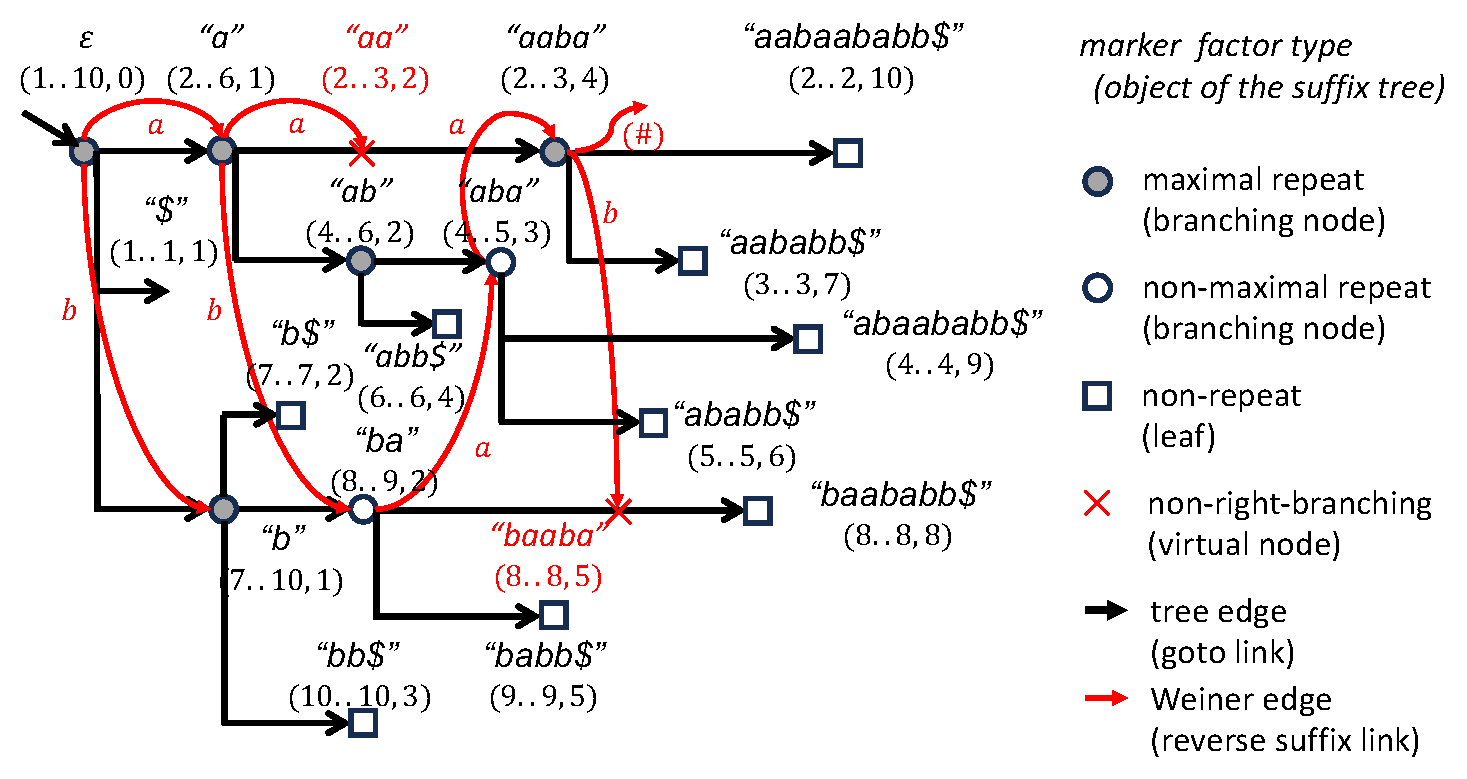
\includegraphics[width=0.7\textwidth]{fig3run.pdf}
\vspace{.75\baselineskip}
\caption{An example run of Algorithm $\RecLPT$ for a string $S = \mathtt{aabaababb\$}$, where the left endmarker $S[0]=\#$ and the related suffixes are omitted. 
}\label{fig:run:example}
\end{figure}
%%%%%%


%%%%%%%%%%%%%%%%%%%%%%%%%%%%%%%%%

%% \subsubsection{Computing a set of right-branching characters}
%% %%% 
%% In \cref{algo:genchildren}, we show a procedure $\GenChildren$ for computing the set of all child ranges of an $\ell$-range, based on precomputed arrays $\LCP, \SA, S$.


%% At the top-level, the procedure is invoked with the triple $\pi = (i..j, \ell_*)$ for a factor of $S$ and the pointer to the set $Children = \emptyset$. At every iteration of $\GenChildren[]$, the following pre-condition must be ensured: $\ell_*$ is the lcp-length of all suffixes in the range $i..j$, namely, $RMQ_{LCP}(i+1, j) = \ell_*$ must hold.

%%       %% \If{ $Children = \op{undef}$ }{
%%       %%   We let $Children$ to be the pointer to a newly created set $\emptyset$. 
%%       %% }



%% \begin{toappendix}
%% By definition, we see that
%% $(i,j,\ell) \in \RR$ if and only if
%% \begin{enumerate*}[(i)]
%% \item $k \in i..j \iff u = S[p..p+\ell-1]$ for all $k$, and
%% \item $\ell = minLCP(i,j)$,
%% \end{enumerate*}
%% where $p = SA[k]$ and $minLCP(i,j)$ denotes the minimum LCP-values of an SA-range $i..j$ defined to be $minLCP(i,j) := \max_{i\le k\le j} lcp(S[p..n])$.

%% \begin{remark}[SA-ranges as a representation of right-maximal factors]
%%   We remark that any SA-range $i..j$ without a length component $\ell$ implicitly represents a right-maximal factor of $S$ as follows. By letting $\ell$ to be the min-lcp value of the range, that is, $\ell := minLCP(i,j)$, we obtain the triple $(i..j, \ell)$ representing a $u = S[p..p+\ell-1]$ of $S$, where $p = SA[k]$ with an arbitrary $k \in i..j$. Then, it is not hard to see that $u$ is rigit-maximal in $S$.
%% \end{remark}
%% \end{toappendix}

%% \subsection{Merging dammy leaves to branching nodes (TBD)}


  
%% %%%%%%
%% \begin{figure}[t]
%% \centering
%% 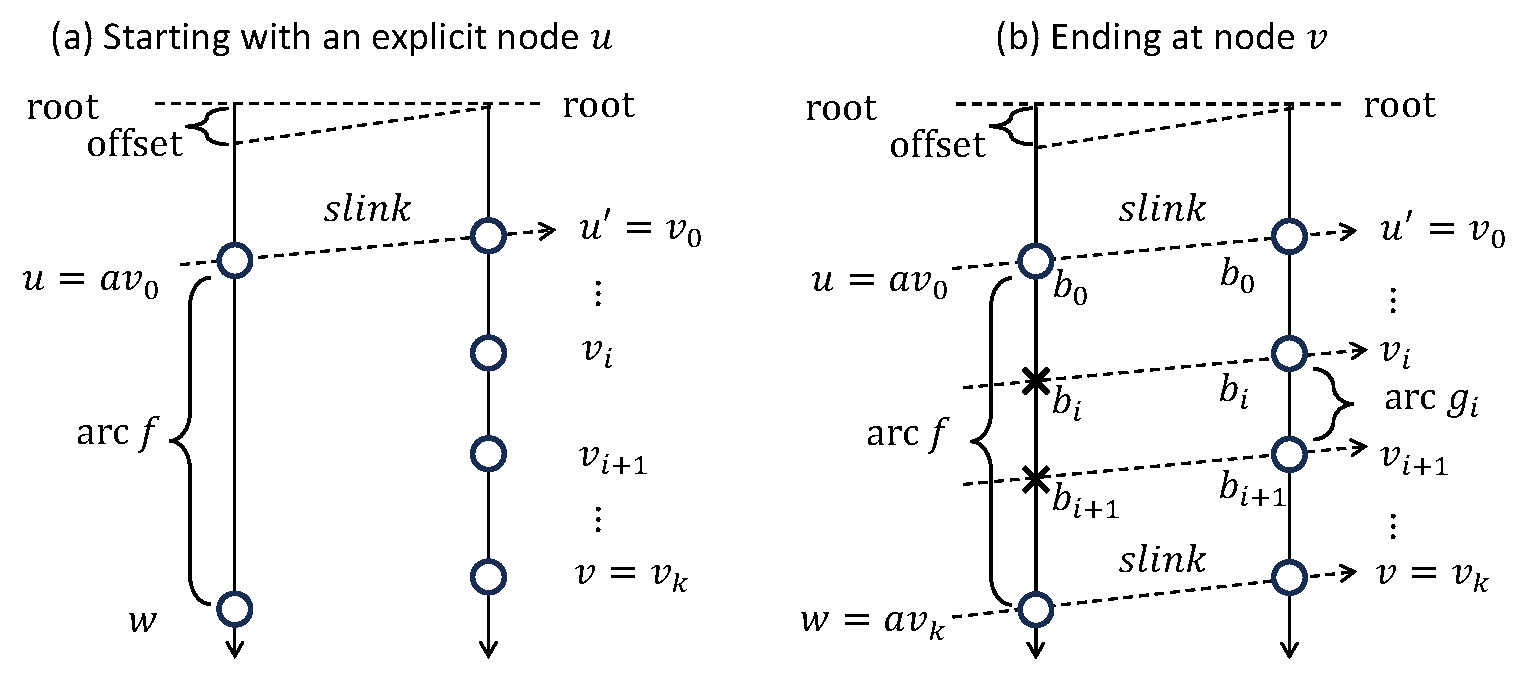
\includegraphics[height=0.4\textwidth]{fig4proof.pdf}
%% \vspace{.5\baselineskip}
%% \caption{Explanation of the procedure $\FindNonEquivLocus(u, \alpha; G, \sdep, \ldep)$ in \cref{algo:find:ne:locus}. Given the string label $\alpha = \lab(f)$ of an arc $f = (u, \alpha, w)$, it finds the locus $v$ of the shrinked string $\alpha' = \alpha[1+\id{offset}..|\alpha|]$. This can be done in total time $O(e_L(S) + e_R(S))$ using the so-called skip-and-count technique.}
%% \label{fig:three:suffix:link}
%% \end{figure}
%% %%%%%%

  

%%%%%%%%%%%%%%%%%%
\section{Transforming \LPTrm-tree to CDAWG}
\label{sec:lpt:to:cdawg}
%%%
In this section, we show how to transform the \LPTrm-tree $T$ of a string $S$ into its CDAWG in $O(e_R(S) + e_L(S)\log\sigma)$ time and $O(e_R(S) + e_L(S))$ space.
In the following, firstly, we briefly review the CDAWG $G$ of a string $S$ according to Crochemore and V\'erin~\cite{crochemore:verin1997direct}. Next, we explain a straightforward algorithm for solving the task in $O(n^2)$ time. After explaining the preprocessing and the working structure that our algorithm uses, we present our algorithm. 

\subsection{Classes of factors and the CDAWG}

Blumer \textit{et al.}~\cite{blumer1987complete} showed that the CDAWG of $S$ is the minimum state DFA of $\Suf$ with path-compression.
%%the properties of the CDAWG $G$ of $S$, 

\mysubsubsection{Classes of factors}
The \textit{syntactic congruence relation associated to end-positions} over $\Fac$, denoted by $\EQe$, is defined, for all $u, v \in \Fac$ by 
\begin{math}
  u \EQe v \iffdef \Epos(u) = \Epos(v). 
\end{math}
Then, the universe of all factors, $\Fac$, is partitioned into the congruence classes $\CLSe{u}$, called \textit{classes of factors}, defined by 
$C(u) = \CLSe{u} := \sete{ v \in \Fac \mid \Epos(u) = \Epos(v) }$
for a factor $u$ of $S$. We call the class of factor $C = C(u)$ \textit{strict} if $u$ is right-branching in $S$, i.e., $\rext{u} = u$. 
The \textit{representative} of $C$ is the longest string in $C$, and is denoted by $value(C)$. 

\mysubsubsection{Representing the CDAWG by classes of factors}
Now, we can describe the CDAWG $G = (V(G), E(G), root(G))$ of $S$ in terms of congruence classes as follows~\cite{crochemore:verin1997direct}.  
Each node of $G$ corresponds to a \textit{strict} class of factor $C$, that is,  $C = C(u)$ with some right-branching factor $u \in \Fac$. The node $C$ represents all factors of $S$ that have the same set of end positions in $S$ as the string labels of all paths from the root to $C$. The root is $C(\eps)$, and there exists an arc $f = (C(u), \alpha, C(v))$ in $E(G)$ if $v = \rext{(ub)}$ and $u\alpha = v$ with some $b \in \Sigma$, called a \textit{branching character}, and $\alpha \in \Sigma^*$. By definition, the string label $\alpha$ starts with the  $b$, i.e., $\alpha[1] = b$.  

\mysubsubsection{Suffix links of the CDAWG}
For any node $u$ in $V(G)$, $G$ has a suffix link $v = \suf(u)$ whose target $v$ is the locus of the longest suffix of $u$ such that $\Epos(v) \not= \Epos(u)$. In other words, the suffix link connects distint classes of factors $C(\alpha v)$ and $C(v)$ by removing a nonempty prefix $\alpha$ of $u = \alpha v$ such that $u = \alpha v$. In what follows, we do not distinguish a class $C(u)$ and its member $u \in C(u)$ if no confusion arises.
For technical reason, we define the string label of a suffix link $\suf(C(\alpha v)) = C(v)$ to be the prefix $\alpha$ satisfying the above condition.%
%%%
\footnote{
Then, the labeled link from $v$ to $\alpha v$ is called a Weiner link, whose label is the last character $a$ of $\alpha$, i.e., $a = \alpha[|\alpha|]$. 
}

%% \subsection{Naive algorithm}


\subsection{Input and output}

An input to our algorithm is the \LPTrm tree $T = (V(T), E(T), root(T))$ of $S$ and the string $S$ itself. In the followings, we identify a factor $u\in \Fac$ and its locus $\underline{u}$ in $T$. We remark that the \LPTrm-tree constructed by the algorithm in \cref{sec:sa:to:lpt} has no suffix links, and from each class of factors, only one rooted-path, namely, the representative path, is chosen. Therefore, our task is to recover these information from $T$. 

We assume that to each node $u$ of $T$, the following information is associated:
\begin{itemize}
\item $\dep(u)\ge 0$: The string depth of $u$, i.e., $\dep(u) = |\str_T(u)|$.
\item $\islb(u) \in \set{\tt true, false}$: The flag indicating whether $u$ is right-branching in $S$, i.e., $|\LC(u)|\ge 2$. 
\item $\parent(u) \in V(T)\cup\set{\op{undef}}$: The parent of $u$ if it exists, and $\op{undef}$ otherwise. 
\end{itemize}

The output is the CDAWG $G$ of $S$, which is obtained from a copy of the input tree $T$ by modifying its structure, and associated with 
the following structures constructed during the computation: 
\begin{itemize}
\item $C: V(T) \to \pow{V(T)}$: A table representing the collection of all and only congruence classes of $V(T)$ supporting the following operations:
  For any clas $C = C(u)$ with $u$,  $C.\op{get}()$ returns the representative of the class $C(u)$, and $C.\op{append}(u)$ adds any $v$ into $C$. We do not need the operation $\op{unify}$.%
%%%  
\footnote{Since the congruence classes form a spanning tree over all factors, the structure is implemented simply by a singley-linked linearly list $L$ of nodes. It linearly grows from the head to the tail by appending a new element to the tail. An extension is that all elments of $L$ has an additional pointer to the head of $L$, as the representave, so that operations are performed in constant time.
}
%%%  
  
\item $\suf: V(T)\setminus{root(T)} \to V(T)$: A table representing the suffix link $\suf(v) = u$ in the CDAWG $G$. 
\end{itemize}

We remark that since $|V(T)|$ and the size of $T$ are upperbounded by $O(e_R(S) + e_L(S))$, so is the above representation of the CDAWG. 


%%%%%%
\begin{figure}[t]
\centering
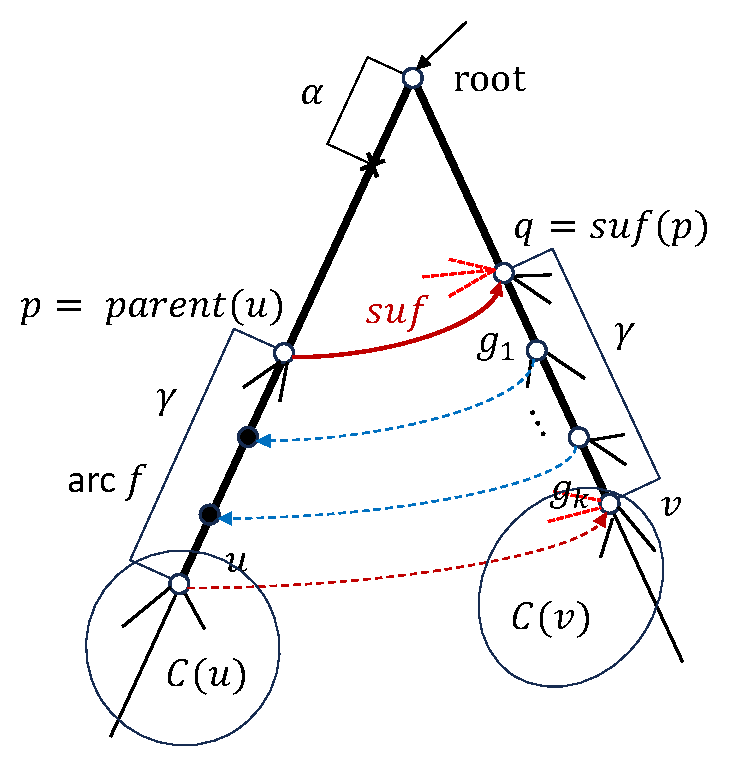
\includegraphics[height=0.4\textwidth]{fig4a.pdf}
%% 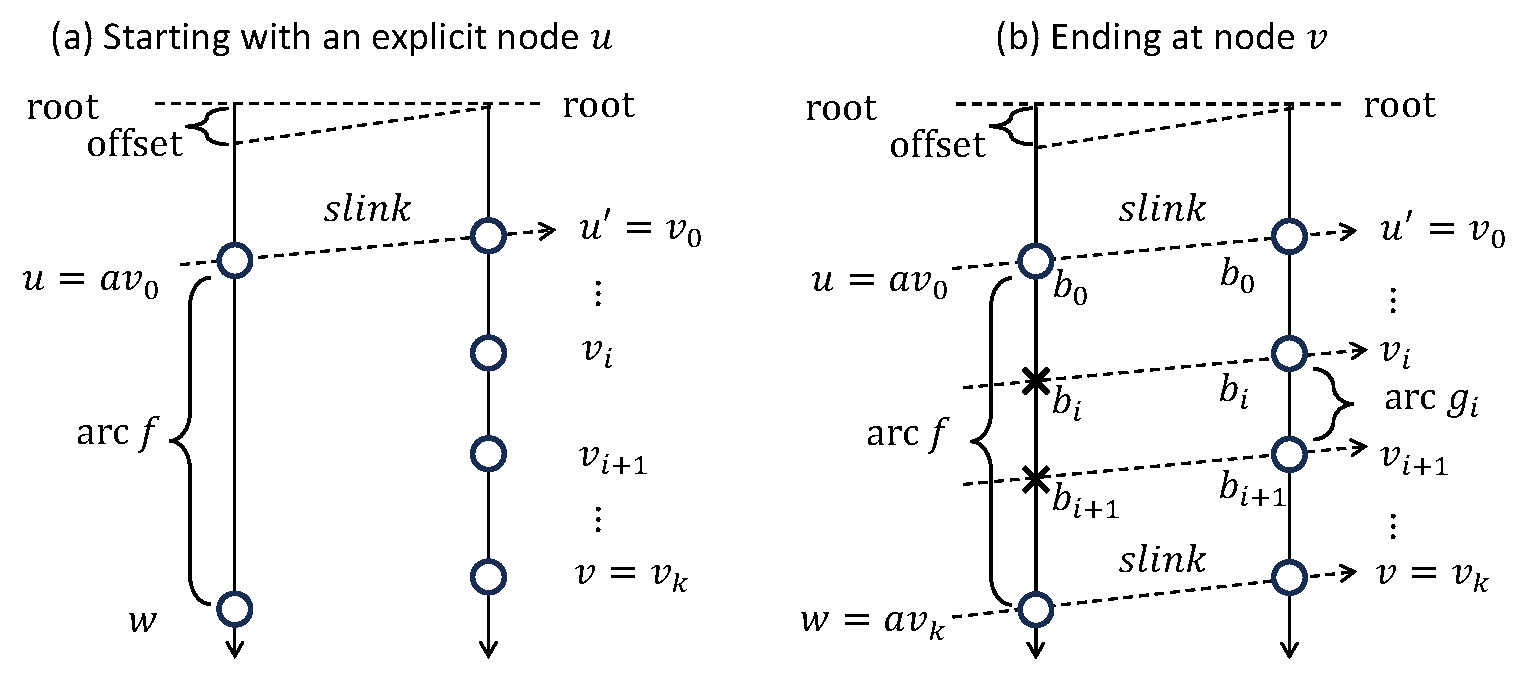
\includegraphics[height=0.4\textwidth]{fig4proof.pdf}
\vspace{.5\baselineskip}
\caption{Explanation of the procedure link-and-merge for transforming the \LPTrm-tree $T$ of a string $S$ into its CDAWG $G$, where white and black circles indicate real nodes and loti. Thick and thin lines indicates solid and non-solid arcs. Given a node $u$ with the minimum $dep(u)$ extracted from a priority queue $B$, it finds the locus of the longest suffix $v$ of $u$ that is not equivalent to $u$ relative to end-positions. Then,
  for two congruence classes $C(u)$ and $C(v)$, 
  it puts a suffix link from $C(u)$ to $C(v)$ if $v$ is left-branching, and merges $C(u)$ and $C(v)$ otherwise. 
}\label{fig:three:suffix:link}
\end{figure}
%%%%%%

\newpage
\subsection{Link-and-Merge Algorithm}
\label{sec:algo:link:merge}

Our algorithm constructs the CDAWG of $S$ from its \LPTrm-tree, based on an idea similar to McCreight's suffix tree construction algorithm~\cite{mccreight1976space} as well as Crochemore and V\'erin's CDAWG construction algorithm from a string $S$~\cite{crochemore:verin1997direct}.

\begin{definition}[high-level description of the procedure for computing suffix links and classes of factors from $\sig L$]\label{lem:maxrep:algo:highlevel}
\begin{enumerate}[(1)]
\item[] \hspace{-.75\leftmargini}\textbf{Procedure} Link-and-Merge: Computing the CDAWG $G$ of a string $S$ from its \LPTrm-tree $T$.
\item For each node $u$ in $V(T)$, insert $u$ with weight $\dep(u)$, i.e., $(u, \dep(u))$, into the priority queue $B$.
\item While $B \not= \emptyset$, do the following steps: 
\begin{enumerate}[(a)]
\item Extract a node $u$ from $B$ with the minimum weight $\dep(u)$, and delete it from $B$. 
\item Find the locus $v$ of the longest suffix  of $u$ such that $\Epos(u) \not= \Epos(v)$.
\item Either merge $C(u)$ and $C(v)$ or commect them by putting a suffix link from  $C(u)$ and $C(v)$, depending on whether $C(u) = C(v)$. 
\end{enumerate}
\end{enumerate}
\end{definition}

In Step (1-c), we check whether $C(u) = C(v)$ holds or not. 



%%%%%%%%%%%%%%%%%%
\begin{algorithm}[t]
  \caption{A procedure $\idsf{RecSuf}$ that implementes the procedure Link-and-Merge for computing the CDAWG $G = (V(G), E(G), \suf, \eps)$ of a string $S$  from the \LPTrm-tree $T = (V(T), E(T), \eps)$ of $S$ in $O(e_L(S) + e_R(S))$ time and space, where a variable $C: V(T)\to \pow{V(T)}$ is a mapping that assigns a class of factors to each node of $T$. 
  }\label{algo:rec:cdawg}
  %%%%%%
  $\suf \gets \emptyset$; 
  $C \gets \emptyset$\;
  Create the virtual parent $m$ of $root$, called the master root,  with outgoing edges $Out(m) = \set{ f = (m, b, root) }_{b \in \Sigma}$ and the suffix link $\suf(root) \gets m$\;
  %% \iFor{$b \in \Sigma$}{
  %%   $Out(m) \gets (m, b, root)$\;
  %% }
  %% $\suf(root) \gets m$\;
  \For{$u \in V(T)$}{
    $\idsf{RecSuf}(u)$\; 
  }
  \medskip
  \textbf{Procedure} $\idsf{RecSuf}(u: \idrm{node})$\; 
  \Begin{
      \uIf{ $\suf(u) \not= \op{undef}$ }{
        $v \gets \suf(u)$\; 
      }
      \Else{
        $p \gets parent(u)$\;
        $q \gets \idsf{RecSuf}(p)$\; 
        $v\gets$ Find the locus $v$ of the longest suffix of $u$ such that $\Epos(u) \not= \Epos(v)$, by skip-and-count from $q$ with string label $\gamma = \lab(g)$ of incoming edge $g = \pair{p, parent(u)}$ of $u$\;
        %% $v\gets \idsf{SkipAndCount}(\gamma)$, where $\gamma = \lab(\pair{p, parent(u)})$\;
        \uIf (\comblk{Case: $C(u) \not= C(v)$}) { $v$ is left-branching }{
          $\suf(u) \gets v$\; 
          \Return $\suf(u)$\; 
        }
        \Else (\comblk{Case: $C(u) = C(v)$}) {
          $C(v).\op{append}(u)$\;
          Redirect all incoming edges of $u$ to $v$\; 
        }
      }
      \Return $v$\; 
    }
\end{algorithm}

%%%%%%%%%%%%%%%%%%%%
\section*{Old Transforming \LPTrm-tree to CDAWG}
\label{sec:lpt:to:cdawg:old}
%%%
In this section, we present the second algorithm $\RecCDAWG$ for transforming the \LPTrm-tree $G = (\sig V(G), \sig E(G), root_G)$ for a string $S$ into its CDAWG.
We show the main result of this section.  

\begin{lemma}\label{lem:main:lpt:to:cdawg}
  Let $S$ be any string of length $n$ over $\Sigma$. 
  We can transform the \LPTrm-tree $T$ of $S$ without suffix links into its CDAWG $G$ with suffix links in $O(e_R(S) + e_L(S))$ time and working space, where $e_R(S)$ and $e_L(S)$ are the numbers of right- and left-extensions of maximal repeats in $S$, and an algorithm is allowed to access the read-only copy of the string $S$. 
\end{lemma}

In the above theorem, we remark that the sizes of an input $T$ and the output $G$ are both $O(e_R(S) + e_L(S))$. 

In \cref{algo:rec:cdawg}, we present the psuedo code of $\RecCDAWG$. 
This algorithm performd the breadth-first search of $T$ from the root to leaves using $\sdep(v)$ as the weight of each node $v$. Then, it gradually transforming an input $T = \LPT(S)$ into a partial DAG obtained from $G = \CDAWG(S)$ by merging equivalent nodes into equivalence classes, and adding suffix links between inequivalent nodes. In the following, we will refer to an itermediate DAG $G'$ as a \textit{partial CDAWG} of $S$. When the merging process is done, the resulting partial DAG $G'$ becomes $\CDAWG(S)$.


In the following subsections, we first explain its subroutines. Finally, we present the proof of \cref{lem:main:lpt:to:cdawg} by analyzing the correctness and time complexity of \cref{algo:rec:cdawg}. 


%% %%%%%%%%%%%%%%%%%%
%% \begin{algorithm}[p]
%%   \caption{The procedure $\RecCDAWG$ for transforming the \LPTrm-tree $T = (V(T), E(T), root(G))$ of a string $S$ into its CDAWG $G$. 
%%   }\label{algo:rec:cdawg}
%% %%%%%%
%%   %%%
%% \KwWork{$B\subseteq V(G)\times \nat$: a priority queue of nodes $u$ with $\ldep(u)$ as their weights. $EQ: V(G) \to \pow{V(G)}$: a union-find structure that maps each vertex $u$ to its equivalence class $EQ(u) \in \pow{V(G)}$ with operation $\op{unify}(u, v)$. Tables $\ldep, \sdep: V(G) \to \nat$ that assigns to each node $u$ the string depths of the longest and shortest members in $EQ(u)$ in $T$, respectively. }  
%% \Begin{ 
%% \Comment{Initialization}
%% $B \gets \emptyset$, $\id{suf} \gets \emptyset$, and $wlink \gets \emptyset$\;
%% Compute the table $\ldep$ by DFS of $T$\; 
%% \For{each $u \in V(G)$}{
%%   $\op{isLB}(u)=|\LC(\Value(u))|$\Comment*{from the triple of $u$} 
%%   $EQ(u) = \set{u}$\Comment*{the singleton class}
%% }
%% \For{each $f = (u, \alpha, w) \in E(G)$}{
%%   $B.\op{insert}(f, \ldep(w))$
%%   \Comment*{Insert $f$ with weight $\ldep(w)\ge 0$}
%% }
%% \medskip
%% \While{ $B \not= \emptyset$}{
%%   \Comment{Extracting an arc with minimum weight $\ldep(w)$}
%%   $f = (u, \alpha, w) \gets B.\op{deletemin}()$\;
%%   \Comment{Finding the locus $v$ of the longest suffix $\beta'$ of the string label $\beta = \Value(u)\cdot\alpha$ such that $\beta' \not\in EQ(\beta)$. }
%%   $(u', (g_1, \dots, g_k), v) \gets \FindNonEquivLocus(u, \alpha; G, \sdep, \ldep)$\; 
%%     \label{step:algo2:skip:and:count}
%%     \Comment{Maintaining links and equivalence class of $v$}
%%     \uIf (\comblk{Merging two equivalence classes})
%%          {$\op{isLB}(v) = 1$}
%%          %% {$|\wlink(v)| = 0$}
%%          {
%%       \Comment{$v$ has no incoming suffix links.}
%%       $EQ.\op{unify}(w, u)$
%%        \Comment*{Merging $EQ(w)$ and $EQ(v)$}
%%       Re-direct all incoming arcs of $v$ into $w$\;
%%       $\sdep(w) \gets \min\{\sdep(w), \sdep(v)\}$\; 
%%     }
%%     \Else (\comblk{Adding suffix and Weiner links between equivalence classes})
%%     {
%%       $a = \alpha[\id{offset}]$\Comment*{$\op{shortest}(EQ(w)) = a\cdot \Value(EQ(v))$}
%%       $\id{suf}(w) \gets v$\Comment*{an incoming suffix link to $v$}
%%       $\wlink(v, a) = v$\Comment*{an explicit W-link from $v$}
%%       %% Add , namely, , and  with character $a$, namely, , where  is the first character of the shortest emember of $EQ(w)$, that is, . \; 
%%     }
%% } %% While
%% \Return the CDAWG $G = (V(T), E(T), root(G), \id{suf}, \wlink)$ of $S$\; 
%% }%Begin
%% %%%%%%
%% \end{algorithm}
%% %%%%%%%%%%%%%%%%%%




%% We show a few technical lemmas below. Let $G'$ be a partial CDAWG obtained from $\LPT(S)$ by merging a subset of equivalent nodes with respect to the equivalence relation $\eqepos$ on $\Fac$. 

%% \begin{lemmarep}\label{lem:trans:cdawg:one}
%% Let $\alpha, \beta \in \Fac$ be any factors of $S$ such that $\alpha$ is a suffix of $\beta$, i.e. $\beta \succeq^\idrm{suf} \alpha$. In $\CDAWG(S)$, if the locus of $\beta$ is an explicit node of $G'$, then so is the locus of $\alpha$. 
%% \end{lemmarep}

%% \begin{proof}
%%   Recall that a locus $\loc u$ is an explicit node in
%%   $\CDAWG(S)$
%%   if and only if
%%   $|\Epos(u)| \ge 2$.
%%   Since $\beta \succeq^\idrm{suf} \alpha$, we have $|\Epos(\alpha)| \ge |\Epos(\beta)| \ge 2$. 
%% \qed\end{proof}

\subsection{Preprocessing $\op{ldep}(u)$ and $\sdep(u)$ in $O(e_R)$ total time}
\label{sec:compute:cdawg:preprocess}

During the computation, we incrementally compute the the pair $(\op{ldep}(u), \sdep(u))$ of quantities on the \LPTrm-tree, defined as follows. 
 %% and $\op{shortdep}(u)$ of the longest and shortest paths from the root to $u$ are already computed, where
\begin{itemize}
\item $\op{ldep}(u)$ is the \textit{largest string depth}, defined to be the length of the longest paths from the root to $u$,
that is, $\ldep(u) = \max \sete{ |\str(\pi)| : \pi \in Path(root, u) }$

\item $\sdep(u)$ is \textit{the smallest string depth}, defined to be the length of the longest paths from the root to $u$, that is, $\sdep(u) = \min \sete{ |\str(\pi)| : \pi \in Path(root, u) }$. 
\end{itemize}

Clearly, $\ldep(u) = |\Value(u)|$.
The fields for the above information require $O(\mu(S))$ space. 
Then, the computation of the the pair $(\op{ldep}(u), \sdep(u))$ is done by the following recurrences. 
\begin{lemma}\label{lem:ldep:sdep:rec}
Let $G$ be the CDAWG  of a string $S$ and $u$ be any of its explicit node. 
\begin{enumerate}
\item If $u$ is the root of $G$, $\ldep(u) = \sdep(u) = 0$. 
  
\item Otherwise, $u$ is an explicit node with one or more incoming arcs $f_1, \dots, f_k$ such that $\dst(f_i) = u$ for all $\btw i1k$ and $k\ge 1$.
Then, we have 
  \begin{itemize}
  \item $\ldep(u) = \max{}\idx i1k \{\: \ldep(\src(f_i)) + |\lab(f_i)|  \:\}$
  \item $\sdep(u) = \min{}\idx i1k \{\: \sdep(\src(f_i)) + |\lab(f_i)|  \:\}$
  \end{itemize}
  where $f_i = (\src(f_i), \lab(f_i), \dst(f_i)) = (v_i, \alpha_i, u) \in V(G)\by\Sigma^+\by V(G)$. 
\end{enumerate}
\end{lemma}

From \cref{lem:ldep:sdep:rec}, the total computation can be done in $O(e_R(S)+e_L(S))$ time and $O(\mu(S))$ working space on the CDAWG of $S$. 
We remark that \cref{lem:ldep:sdep:rec} holds even for a partial CDAWG $G$ whenever the current node $u$ has been merged to all of its equivalent nodes and all ancestors have been processed so far.

  We assume that the Boolean flag $\op{isLB}(v) \iffdef |\LC(\Value(v))|\ge 2$ is attached to each explicit node $v$ in $T$. This can be  computed from the triple for $\Value(v)$ by $\isLeftBranching(i..j, \ell)$ of \cref{lem:leftmaximal:character} in the procedure $\RecLPT$. 



%%%%%%%%%
\subsection{Computation of the locus of the longest non-equivalent prefix of the representative string}
\label{sec:compute:cdawg:equiv:classes}
%%
In the CDAWG of $S$, there exists a suffix link between the representatives $\beta$ and $\beta'$ of two equivalence classes such that $|\beta| > |\beta'|$ if and only if $\beta'$ is the longest suffix of $\beta$ that does not belong to the equivalence class of $\beta$.
Therefore, it is sufficient to find the locus $v$ of such $\beta'$ from the locus $w$ of $\beta$. Then, we have the next lemma. 


\begin{lemma}\label{lem:find:ne:locus}
  %%\textit{Claim}~2.
  During the computation of a partial CDAWG of $S$ from $\LPT(S)$, 
  the computation of the target $v$ and the arcs $g_1, \dots, g_k$ can be done in $O(e_R(S)+e_L(S))$ total time over all arcs $f$ using the procedure  $\FindNonEquivLocus$ in \cref{algo:find:ne:locus}. 
\end{lemma}


\begin{toappendix}
In \cref{algo:find:ne:locus}, we show the procedure $\FindNonEquivLocus(u, \alpha; G, \sdep, \ldep)$ that computes the locus $v$ of the longest suffix $\beta'$ of the string label $\beta = \Value(u)\cdot\alpha$ such that $\beta' \not\in EQ(\beta)$, and the associated path $(g_1, \dots, g_k)$ from a node $u'$ to $v$.
See \cref{fig:three:suffix:link} for the explanation of the procedure.

%%%%%%%%%%%%%%%%%%
\begin{algorithm}[t]
  \caption{
The procedure $\FindNonEquivLocus(u, \alpha; G, \sdep, \ldep)$ that computes the locus $v$ of the longest suffix $\beta'$ of the string label $\beta = \Value(u)\cdot\alpha$ such that $\beta' \not\in EQ(\beta)$, and the associated path $(g_1, \dots, g_k)$ from a node $u'$ to $v$. 
  }\label{algo:find:ne:locus}
  %%%%%%
  \Comment{Computing the initial node $u'$ and a suffix $\alpha'$ of $\alpha$}
  \uIf{$u = root(G)$}{
    $(u', \id{offset})\gets (root(G), 1)$\; 
  }
  \Else{
    $(u', \id{offset})\gets (\id{suf}(u), \ldep(u) - \sdep(u) + 1)$\; 
  }
  $\alpha' \gets \alpha[\id{offset}..|\alpha|]$\; 
  %%%
  %%At stage $i=0$, we initialize the target length by
  \Comment{Finding a path $(g_1, \dots, g_k)$ with skip-and-count}
  $\ell_* \gets |\alpha|$; $\ell \gets 0$; $v_0 \gets v$; $i \gets 0$\;     
  \While{$\ell < \ell_*$}{
    $b_i \gets \alpha[\ell + 1] \in \Sigma$\Comment*{a branching character}
    $g_i = (v_{i-1}, \beta_i, v_i) \gets \Out(v_{i-1}, b_i)$\; 
    $\wlink(v_i, a) \gets f$\Comment*{Adding a new implicit W-link}
    $\ell \gets \ell + |\beta_i|$; $i \gets i+1$\; 
  }
  \Return $(u', (g_1, \dots, g_k), v)$, where $k = i-1$\; 
\end{algorithm}
%%%%%%%%%%%%%%%%%%
\end{toappendix}

\section{Analysis}
\label{sec:analysis}
%% \subsection{The proof of \cref{lem:main:lpt:to:cdawg}}

Consider the psuedo code of the procedure $\RecCDAWG$ in \cref{algo:rec:cdawg}. To prove its correctness, we define  
  $\eqepos[\preceq w]$ and $[u]^{\prec w}_{\equiv}$ to be the restriction of
  the equivalence relation $\eqepos[]$ and class $\eqepos[\prec w]$
  onto the subset of nodes $v$ such that $\ldep(v) \le \ldep(w)$.
  Similarly, we use subscript $\cdot^{\prec w}$ for the version of $\ldep(v) < \ldep(w)$.


\begin{lemmarep}[correctness]\label{lem:cdawg:correctness}
  Let $T$ be the $\LPT(S)$ of a string $S$ of length $n$. 
  We assume that the Boolean flag $\op{isLB}(v)$ is attached to each explicit node $v$ in $T$. Then, \cref{algo:rec:cdawg} correctly computes $\CDAWG(S)$ from $T$ and $S$. 
\end{lemmarep}

\begin{proofsketch}
  The proof is done by induction on the iteration of the while-loop of \cref{algo:rec:cdawg} and target $w$ of a new arc $f = (u, \alpha, w)$ extracted from queue $B$ at Line 10. 
  We let $v$ be the deepest node in $V\rk{\prec w}(T)$ such that
  $\beta \not\eqepos[\prec w] \beta'$
  %$[v]^{\prec w}_{\equiv} \not= [w]^{\prec w}_{\equiv}$
  and $\beta \succeqsuf \beta'$ (*)
  with $\beta = \Value(w)$ and $\beta' = \Value(v)$ 
  in the beginning of the while-loop. This (*) means that the equivalence classes of $w$ and $v$ are different. 
  Such a $v$ always exists for $v = root(T)$, and 
  can be found by $\FindNonEquivLocus$ from \cref{lem:find:ne:locus}. 
  There are two cases (a) and (b) to maintain the current $\eqepos[\preceq w]$:
\begin{enumerate*}[(a)]
\item The case that $\beta \eqepos[\preceq w] \beta'$ holds, and $|\LC(\beta')| = \op{isLB}(v) \ge 2$, detected at Line 10. Then, two equivalence classes must be merged into a new class. 
  %% the equivalence classes $[w]^{\prec w}_{\equiv}$ and $[v]^{\prec w}_{\equiv}$ of $\beta$ and $\beta'$, respectively, must be merged into the new class $[w]^{\preceq w}_{\equiv}$. This is done by the code for Lines 11--13. 
\item The case that $\beta \not\eqepos[\preceq w] \beta'$ holds, and $|\LC(\beta')| = \op{isLB}(v) = 1$, detected at Line 14. Then, the suffix link from $w$ to $v$ must be added, where $\id{offset} = |\beta| - |\beta'|$ and $a = \alpha[\id{offset}]$. 
\end{enumerate*}
Therefore, Lines~12--19 correctly update the equivalence class $EQ(w)$ for $[w]^{\prec w}_{\equiv}$, $\id{suf}$, and $\id{wlink}$. If \cref{algo:rec:cdawg} exits the while-loop, the resulting DAG $G$ with $EQ, \id{suf}$, and $\id{wlink}$ becomes $\CDAWG(S)$. Hence, the result is proved.
\qed
\end{proofsketch}

\begin{proof}
Suppose that initialization of Lines 2--6 are done. 
We introduce some notion as follows.
Consider any iteration of the while-loop for Lines 7--17 of \cref{algo:rec:cdawg}.
Let $w$ be any explicit node in $V(T)$.
\begin{itemize}
\item We define the total order $\preceq$ on $V(G)$ as $u \preceq v \iffdef \ldep(u) \le \ldep(v)$, and its strict version $\prec$. 
\item For any explicit node $w$, we denote $V\rk{\preceq w}(T) := \sete{ v \in V(T) \mid \ldep(v) \le \ldep(w) }$ be the subset of all nodes $v$ with $\ldep(v) \le \ldep(w)$.
  
\item We let $\eqepos[\preceq w]$ be the subrelation of $\eqepos$ restricted to $V\rk{\preceq w}(T)$, namely, $(\eqepos[\preceq w]) = \sete{ (u,v) \in (\eqepos) \mid u, v \in V\rk{\preceq w}(T)}$, and $[u]^{\preceq w}_{\equiv}$ be the associated equivalence class with representative $u$.

\item Similarly, we let $\eqepos[\prec w]$ and $[u]^{\prec w}_{\equiv}$ as the subrelation and equivalence class with $\prec w$ instead of $\preceq$, respectively. 
\end{itemize}

At the timing where a new arc $f = (u, \alpha, w)$ with weight $\ldep(w)$ is extracted from $B$, we remark that $\eqepos[\prec w]$ and $\eqepos[\preceq w]$ correspond the node subsets $V\rk{\preceq w}\setminus\set{w}$ and $V\rk{\preceq w}(T)$, respectively. We will show the following claim.

\textit{Claim~1}: At any iteration of the while-loop for Lines 7--17 of \cref{algo:rec:cdawg}, suppose that a new arc $f = (u, \alpha, w)$ with weight $\ldep(w)$ is extracted from the priority queue $B$. Then, in the end of the iteration at Line 17, the following conditions hold:  
\begin{enumerate}
  \item For all explicit nodes $w'$ in $V\rk{\preceq w}(T)$ with $\ldep(w') \le \ldep(w)$, $EQ(w') = [w']^{\preceq w}_{\equiv}$ holds and $w'$ has an outgoing suffix link.
  \item For all explicit nodes $w'$ with $\ldep(w') < \ldep(w)$, $w'$ has a soft-Weiner link $\wlink(w', a) = g$ for some character $a$ and an arc $g$ if the string $a\cdot\Value(w')$ is a factor of $S$. 
\end{enumerate}


Consider condition (1). Let $f = (u, \alpha, w)$ be the new arc with weight $\ldep(w)$ is extracted from $B$ in the beginning of the while-loop.
We will show the claim that at the end of the while-loop, the equivalence relation $\eqepos[\preceq w]$ and the associated equivalence classes are correctly maitained on the updated domain $V\rk{\preceq w}(T) = V\rk{\prec w}(T) \cup \set{w}$. 

Suppose first that there exists another node $v$ in $V\rk{\prec w}(T)$ such that $[v]^{\prec w}_{\equiv} \not= [w]^{\prec w}_{\equiv}$ and $\Value(w) \succeqsuf \Value(v)$ (*) in the beginning of the while-loop. Note that we use $\prec w$ instead of $\preceq w$. Then, we see that $\ldep(v) < \ldep(w)$ othewise they must be identical. 
Among such $v$'s, we choose the deepest $v$ with largest $\ldep(v)$ in $V\rk{\preceq w}(T)$ with property (*).
From \cref{lem:find:ne:locus}, we can find the locus $v$ by calling $\FindNonEquivLocus$ with arguments $u$ and $\alpha$ at Line~9 of \cref{algo:rec:cdawg}. 
%%we can find such a node $v$ with the string label $\beta' = \Value(v)$ by using the procedure $\FindNonEquivLocus$. 


Let $\beta$ and $\beta'$ be the string labels of $w$ and $v$, respectively. Then, we can show that $\beta'$ is the longest suffix of $\beta$ such that $\Epos(\beta) \not= \Epos(\beta')$.
There are two cases (a) and (b) below on the current equivalence relation $\eqepos[\preceq w]$ instead of $\eqepos[\prec w]$. 
\begin{enumerate}[(a)]
\item If $\beta \eqepos[\preceq w] \beta'$ holds, since $\beta \succsuf \beta'$, we can show that this condition is equivalent to $|\LC(\beta')| = \op{isLB}(v) \ge 2$, which can be correctly detected at Line 10. 
  the equivalence classes $[w]^{\prec w}_{\equiv}$ and $[v]^{\prec w}_{\equiv}$ of $\beta$ and $\beta'$, respectively, must be merged into the new class $[w]^{\preceq w}_{\equiv}$. This is done by the code for Lines 11--13. 
  
\item Otherwise, $\beta \not\eqepos[\preceq w] \beta'$ holds. By the same argument as (a), this condition is equivalent to $|\LC(\beta')| = \op{isLB}(v) = 1$, which can be correctly detected at Lines 10 and 14.
  the equivalence classes $[w]^{\prec w}_{\equiv} = [w]^{\preceq w}_{\equiv}$ and $[v]^{\prec w}_{\equiv} = [v]^{\preceq w}_{\equiv}$  of $\beta$ and $\beta'$, respectively, must remain separated, and the suffix link from $w$ to $v$ must be added, where $\id{offset} = |\beta| - |\beta'|$ and $a = \alpha[\id{offset}]$. 
  This is correct because $[v]^{\prec w}_{\equiv}$ is the predecessor of $[w]^{\prec w}_{\equiv}$ w.r.t.~the suffix relation $\succsuf$ on their values.
\end{enumerate}

Combining the above arguments, at the end of the while-loop, we have correctly maintained the equivalence relation $\eqepos[\preceq w]$ and the associated equivalence clases on the updated domain $V\rk{\preceq w}(T) = V\rk{\prec w}(T) \cup \set{w}$.
\qed\end{proof}

Combining the above discussion, we give the proof for main results. 

%% Next, we consider the time complexity. 

\begin{lemmarep}[time and space complexity]\label{lem:cdawg:complexity}
  Given $\LPT(S)$ of a string of length $n$, 
  \cref{algo:rec:cdawg} runs in $O(e_R(S) + e_L(S) + \mu(S)\log \mu(S))$ time and $O(e_L + e_R)$ space. 
\end{lemmarep}

\begin{proof}
Let us denote by $\mu = \mu(S), e_R = e_R(S)$, and $e_L = e_L(S)$, where $\mu \le \min\{e_R, e_L\}$.
In the initialization for the tables $EQ$, $\ldep$, $B$ for Lines 2--8 can be done in $O(e_R)$ total time. The precomputation of the table $\op{isLB}$ at Lines 7--8 can be done in $O(e_L)$ total time by computing $\LC(\tau)$ with the associated triple $\tau$ stored in $u$. 
In each iteration of the while-loop, $\op{deletemin}$ on the priority queue requires $O(\mu \log \mu)$ total time over all of $\mu$ nodes using $O(\mu)$ space on the standard heap.
From \cref{lem:find:ne:locus}, the call of $\FindNonEquivLocus$ at Line~9 requires $O(e_R + e_L)$ total time. Redirection of all incoming arcs of $v$ into $w$ at Line 13 can be done in $O(e_R)$ since $v$ has exactly once suffix link since it is equivalent to $w$, and thus it is not left-branching.
Additions of the suffix and Weiner links for Lines 18--19 can be executed at most the number of suffix links, and are bouned in $O(e_L)$ time.
\qed\end{proof}

\begin{trivlist}\item[]
  \textbf{Proof of \cref{lem:main:lpt:to:cdawg}:}
  From \cref{lem:cdawg:correctness} and \cref{lem:cdawg:complexity}. 
\qed   
\end{trivlist}

\begin{trivlist}\item[]
  \textbf{Proof for \cref{thm:main:index:cdawg}}.
  From 
  \cref{lem:main:from:lpt:to:cdawg:correct:time}
  and
  \cref{lem:main:lpt:to:cdawg}. 
\qed
\end{trivlist}



%% In \cref{algo:rec:cdawg}, we present the psuedo code of $\RecCDAWG$, which gradually transforms $T = \LPT(S)$ to $G = \CDAWG(S)$ by performing breadth-first search of $T$ from the root to leaves. 
%% During BFS, it adds suffix links between inequivalent nodes and merges equivalent nodes into equivalence classes. 
%% %% Our algorithm incrementaly computes suffix links and equivalence classes by
%% %% performing depth-first search from the root to leaves in the \LPTrm-tree. 
%% We will refer to an itermediate DAG $G'$ obtained form the \LPTrm-tree after merging a subset of equivalent nodes as a \textit{partial CDAWG} of $S$. When the merging process is done, the resulting partial DAG $G'$ becomes $\CDAWG(S)$.

%% Below, we show the details of \cref{step:algo2:skip:and:count} in the above algorithm. The traversal can be done in $O(k)$ time using constant time per arc, by the skip-and-count technique as follows (see \cref{fig:three:suffix:link}).e

%% %%%%
%% \begin{enumerate}
%%   \item  
%%     Select the triple $(v, \id{offset}, \alpha')$ of the initial node $v \in V(G)$, a positive integer $\id{offset} \in \nat$, and a prefix $\alpha'$ of $\alpha$ as follows. Let $u = \src(f)$ be the source of arc $f$: 
%%     \begin{enumerate}[(i)]
%%     \item If $u$ is the root, we let $v := root(G)$, and $\id{offset} := 1$. 
%%     \item Otherwise, $u$ is an explicit node other than the root, with the suffix link $\id{suf}(u)$. Moreover, the pair $(\ldep(u), \sdep(u))$ has been computed. Then, we let $v$ to be the target of the suffix link, $v := \id{suf}(u)$, and let $\id{offset} := \ldep(u) - \sdep(u) + 1$. 
%%     \end{enumerate}
%%     Finally, we shrink the label of $\alpha$ by $\id{offset}$ character length, that is, $\alpha' := \alpha[1+\id{offset}..|\alpha|]$.
%%     The intended meaning of $\alpha'$ is the longest suffix of the representative $\Value(u)$ that do not belong to the equivalence class of $u$.
%% \end{enumerate}
%% %%%%



%% %%%%%%%%%
%% \subsection{$O(e_R)$-time Computation of the Equivalence Classes}
%% \label{sec:compute:cdawg:equiv:classes}
%% %%% 
%% %%Then, the algorithm computes the suffix link of explicit nodes, and all inplicit W-links into all type-2 nodes (loti) by breadth-first traversal of the \LPTrm-tree. We make the following inductive assumption. 
%% %We first performs the base case, and then induction cases. Finally, return the revised graph $G = (\sig V, \sig E, root, \wlink, \id{suf})$.

%% In \cref{line:recdag:one}, by induction hypothesis, $w$ is an explicit node whose target $w$ has the smallest string depth $\ell = \ldep(w)$ among the targets of all unprocessed arcs in $B$. This implies the next claim. \; 
%% \begin{enumerate}[(1)]
%%   \item 
%%     \begin{itemize}
%%     \item \textit{Claim}~1. All node in $V(T)$ with string length strictly less than $\ell$ are already processed as follows. If $u$ is not the root, it has a suffix link $\id{suf}(u)$ to another explicit node. Furthermore, it is already merged into the equivalence class $EQ(u')$ of a smaller string depth $\ldep(u')$ equivalent to $u$, i.e., $u \eqepos u'$. 
%%     \end{itemize}
%% \end{enumerate}



%% %%%%%%
%% \mysubsubsection{The base case. We perform the following initialization.}
%% %%%
 
%% \begin{itemize}
%% \item We let $B \gets E(G)$, $suf \gets \emptyset$, and $wlink \gets \emptyset$.
  
%% \item For all nodes $u$ in $V(G)$, we let $EQ(u)$ be the singleton class, i.e., $EQ(u) = \set{u}$. 
%% %% \item Insert all outgoing arcs $f \in \Out(root(G))$ of the root into $B$ with weight $w = \ldep(\dst(f))$.
%% \end{itemize}

%% \mysubsubsection{The induction case.}
%% %%%
%% As induction hypothesis, we assume that whenever an edge $f \in \sig E(G)$ is extracted from the queue $B$, its source $u = \src(f)$ satisfies that: either (i) the source $u$ is the root of $G$, or (ii) $u$ has the suffix link $v = \id{suf}(u)$ with some $v \in \sig V(G)$.
%% Then, we process all arcs in $\sig E(G)$ by executing the following steps while $B \not= \emptyset$: 
%% \begin{enumerate}[(1)]
%%   \item 
%%     Firstly, we extract from the priority queue $B$ a new edge $f = (u, \alpha, w)$ with the minimum weight $\ldep(w)$.
%%     By induction hypothesis, $w$ is an explicit node whose target $w$ has the smallest string depth $\ell = \ldep(w)$ among the targets of all unprocessed arcs in $B$. This implies the next claim. 
%%     \begin{itemize}
%%     \item \textit{Claim}~1. All node in $V(T)$ with string length strictly less than $\ell$ are already processed as follows. If $u$ is not the root, it has a suffix link $\id{suf}(u)$ to another explicit node. Furthermore, it is already merged into the equivalence class $EQ(u')$ of a smaller string depth $\ldep(u')$ equivalent to $u$, i.e., $u \eqepos u'$. 
%%     \end{itemize}
%%     Let $\beta = \Value(u)\cdot \alpha$ the string label of the longest path from the root to $w$ through the arc $f$. Then, if $w$ is an explicit node, then so is $v$ since 
%%     Note that we do not explicitly compute the string label $\beta$.

%%   \item 
%%     Next, we let $\beta'$ be the longest suffix of $\beta$ such that $\beta'$ is not included in the equivalence class $EQ(\beta)$ of $\beta$. Then, we can quickly find the locus $v$ of $\beta'$ by traversing the list of consecutive arcs arcs $g_1, \dots, g_k$ spelling the string label $\lab(g_1)$ $\cdots$ $\lab(g_k) = \beta'$ along the unique path from the root to the locus $v$ of the prefix $\beta'$. 
%%     \label{step:algo2:skip:and:count}
%%     \begin{itemize}
%%     \item \textit{Claim}~2. The computation of the target $v$ and the arcs $g_1, \dots, g_k$ can be done in $O(e_R(S)+e_L(S))$ total time over all arcs $f$ as shown later.
%%     \end{itemize}

%%   \item Finally, we maintain the suffix link and equivalence class of $v$ as follows.
%% By induction hypothesis, we know that the node $v$ is already processed since $\ldep(v) < \ldep(w)$. Then, there are two cases below on the number of suffix links incoming to the target $v$ (this can be checked by $|\wlink(v)|$). 
%%    \begin{enumerate}[(a)]
%%    \item In the case that $|\wlink(v)| = 0$, namely, $v$ has no incoming suffix links. Then, we merge $v$ into the target $w$ of arc $f$ by re-directing all incoming arcs of $v$ into $w$. Moreover, we update the length $\sdep(w)$ of the shortest path to $w$ with $\min\{\sdep(w), \sdep(v)\}$. 

%%    \item Otherwise, add an incoming suffix link to $v$, namely, $suf(w) = v$, and an explicit W-link from $v$ with character $a$, namely, $\wlink(v, a) = t$, where $a = \alpha[\id{offset}]$ is the first character of the shortest emember of $EQ(w)$, that is, $\op{shortest}(EQ(w)) = a\cdot \Value(EQ(v))$. 

%%    %% \item Finally, in both cases, we add all arcs $f'$ outgoing from $v$ into $B$ with the weight $\ldep(\dst(f'))$.
%%    \end{enumerate}
%%   \end{enumerate}
%% %%%%%%


%% %Computation of suffix and Weiner links 
%% %%%%%%

%% \begin{remark} In (2) (iii) (b), This search for a $b_i$-arc always succeeds. 
%% \end{remark}

%% \begin{proof}
%%   We can show the next claim by construction of $\LPT(S)$. 
  
%%   \textit{Claim~1.} Consider $a u \in L(G)$ for some $a \in \Sigma$ and $u \in \Sigma^*$. If $u \not\in L(G)$, then there exists some factorization $u = pq$ with some $p, q \in \Sigma^*$ such that prefix $p$ is equivalent to $ap$, i.e., $\Epos(ap) = \Epos(p)$. (End of Claim~1)

%% In Claim~1, the prefix $p$ is not left-brancing since we have a left-extension $ap$ of $p$ with the same end-positions. Therefore, the traversal from the initial node $v$ to $u = pq$ terminates at the locus of $p$ when the mergi of $\loc p$ into $\loc {ap}$ happened. 
%% \qed\end{proof}





%% Consider the extended LPT tree of $S$, $\LPT(S) = (\sig V(S), \sig E(S), \eps)$. We introduce the set $\sig W(S)$ of Weiner-links as follows. 
%% For any node $\underline u \in \sig V(S)$ with string labels $u$, and any character $a \in \Sigma$, if $v = au$ is a factor of $S$, $au \in \Fac$, we put the (either soft or hard) Weiner link $g = (\underline u, \underline v)$ from $\underline u$ to the locus $\underline v$ of $v$ with character label $\lab(g) = a$ in $\LPT(S)$. Then, we say that $u$ is the parent of $v$, and $v$ is a child of $u$ w.r.t.~$\sig W(S)$. 
%% Moreover, the link $g$ is \textit{hard} if $\underline v$ is a real (right branching) node, and \textit{soft} otherwise (that is, $\underline v$ is a locus on an arc).
%% %% 
%% We can easily show that the total number of hard and soft Weiner links are upperbounded by the number $e_L$ of left-extensions of maximal repeats of $S$. 

%% Without loss of generality, we identify the triples and the nodes of $\LPT(S)$. Based on the above definition of $\sig W(S)$ and its parent-child relation, we show the next lemma, which is the dual of \cref{lem:prune:leftbranch}. 

%% \begin{lemma}\label{lem:prune:rightbranch}
%% Suppose that a triple $\pi$ is the parent of a triple $\tau$ with respect to the Weiner links in $\sig W(S)$. If the factor $au$ defined by $\tau$ is right-branching, the factor $u$ defined by $\pi$ is also right-branching. 
%% \end{lemma}

%% \begin{proof}
%%   By symmetry, the lemma follows from the proof of \cref{lem:prune:leftbranch}. 
%%   %% If $v = au$ for some $a \in \Sigma$, we can easily show that
%%   %% $\RC(au) \subseteq \RC(u)$, and thus that $|\RC(au)| \le |\RC(u)|$. On the other hand $au$ is right-brancing in $S$ if and only if $2\le |\RC(au)|$. It immediately follows that $2 \le |\RC(u)|$ meaning that $u$ is right-brancing in $S$. This shows the lemma. 
%% \qed\end{proof}

%% Recall that $\sig V$ is the set of nodes for all maximal repeats in $\MR(S)$ and $\eps \in \sig V$. 
%% We let $\sig W$ to be the set of all Weiner links $g = (\underline u, \underline{au})$ that connect elements of $\sig V$ with a character $a \in \Sigma$, that is, $\set{u, au} \subseteq \MR(S)$.

%% Now, we define the \textit{Weiner-link counterpart} of $\LPT(S)$, denoted by $\LPT[-](S) = (\sig V_-, \sig W_-, \eps)$ as follows.
%% \begin{itemize}
%% \item $\sig F_- = \sete{ g = (\underline u, \underline au) \mid u\in\MR(S), u\not\in \MR(S) }$ is the set of all Weiner links $g = (\underline u, \underline au)$ that connect maximal nodes of $\sig V$ to non-maximal nodes. 
%%   %%, that is, $u\in\MR(S)$ and $u\not\in \MR(S)$.
%% \item Let $\sig V_- = \sig V \cup \Delta_-$, 
%%   where $\Delta_- = \sete{\underline{au} \not\in\sig V \mid g = (\underline u, \underline{au}) \in \sig F_-}$ be the set of non-maximal nodes reachable from $\sig V$ by arcs of $\sig F_-$.
  
%% \item $\sig W_+$ be the union of $\sig W$ and $\sig F_-$. 
%% \end{itemize}

%% Then, the extend LPT tree w.r.t.~Weiner links in $\sig W$ is the rooted tree $\LPT[-](S) = (\sig V_-, \sig W_-, \eps)$. 


%% \subsection{Putting it all together}
%% %%%

%% Suppose that an index $\sig I = (\SA, \ISA, \LCP, S)$ is preprocessed from $SA$ and $S$ in \cref{algo:main}. 
%% Consider the recursive procedure $\RecLPT$ in \cref{algo:rec}, which is equipped with subprocedure $\GenChildren$ in \cref{algo:genchildren} and the procedure $\isLeftBranching(i..j, \ell)$ in \cref{lem:leftmaximal:character}. 

%% \subsection{$O({e_R(S) + e_L(S)})$-worst-case time solution over a constant alphabet}

%% From
%% \cref{lem:maxrep:howto:child},
%% \cref{lem:genchildren},
%% \cref{lem:leftmaximal:character},
%% and the construction of $\LPT(S)$, 
%% the recursive procedure $\RecLPT$ in \cref{algo:rec} correctly construct all nodes and edges of $\LPT(S) = (\sig V(S), \sig E(S), \eps)$ by generating all maximal repeats by starting with the root $\eps$, and by following all arcs $(u, v)$ in $\E(S)$ defined with the right-closure $v = \rext{(ub)}$ of a right-extension $ub$ with a branching character $b$ using a depth-first traversal of $\LPT(S)$.
%% From \cref{lem:prune:leftbranch}, we see that if it eventually reaches a non-maximal node in $\Delta(S)$, it correctly stops the search and backtracks. Each arc is added to the arc set whenever it is traversed. Since each node $\underline v$ in $\E(S)\cup \F(S)$ can be reached through exactly one incoming arc, the procedure correctly find all arcs.

%% In summary, to the best of our knowledge, however, it remains an open question whether the CDAWG can be computed from the SA and LCP arrays in output-sensitive manner.
%% Specifically, it is not known if this can be done using $O({e_R(S) + e_L(S)})$ or less time and working space --- in addition to the $O(n)$-size read-only inputs --- for repetitive string with right-extension parameter ${e_R(S) + e_L(S)} \le n$.
%% On the other hand, the proposed algorithm in this paper shows that it is possible to perform translation from the SA and LCP arrays into the CDAWG in output-sensitive time and space by a novel combination of known techniques.  


%% \section{Related work}
%% %%% 
%% It is well-known that the problem of transforming the suffix array of a string $S$ into its suffix tree $T$ can be solved in $O(n)$ time and space. This is achieved using the suffix array (SA) and the longest common prefix array (LCP)  with an auxiliary stack of size $\idrm{height}(T)$.
%% This transformation can be performed by simulating either
%% a bottom-up traversal of the suffix tree, as shown by Kasai \textit{et al.}~\cite{kasai:lee2001lcp:linear} and Crochemore \textit{et al.}~\cite{crochemore2021book125problems:chap:satostree}, or
%% a top-down traversal as demonstrated by Abouelhoda, Kurtz, and Ohlebusch~\cite{abouelhoda2004replacing}.

%% Besides this, most closely related work is recent development of $O(n)$-time transformation algorithms for enumeration of \textit{maximal repeats} of a string $S$ using the \textit{Burrows-Wheeler transform} (BWT), 
%% %%augmented with the \textit{Wavelet tree}.
%% which simulate a top-down traversal of the tree of the reversed suffix links, called the \textit{Weiner tree}~\cite{beller:berger2012space:efficient:bbo,nishimoto:cpm2021enum}. 
%% Since the set of maximal repeats corresponds the node set of the CDAWG of the string, they can be expected to be used as a building block to solve the CDAWG construction problem, too. The latest of them, proposed by Nishimoto and Tabei~\cite{nishimoto:cpm2021enum}, runs in $\Theta(n)$-time and $O(r\,\idrm{polylog}(n))$-space based on the r-index~\cite{gagie:navarro:prezza2020fully}.  

%% Recently, Cleary and Dood~\cite{cleary2023constructing} proposed an algorithm for constructing the CDAWG of a string in the form of a grammar using the SA-intervals of maximal repeats of the string. However, they did not mention how to compute such SA-intervals in $O({e_R(S) + e_L(S)})$ time and space. 

%% In summary, to the best of our knowledge, however, it remains an open question whether the CDAWG can be computed from the SA and LCP arrays in output-sensitive manner.
%% Specifically, it is not known if this can be done using $O({e_R(S) + e_L(S)})$ or less time and working space --- in addition to the $O(n)$-size read-only inputs --- for repetitive string with right-extension parameter ${e_R(S) + e_L(S)} \le n$.
%% On the other hand, the proposed algorithm in this paper shows that it is possible to perform translation from the SA and LCP arrays into the CDAWG in output-sensitive time and space by a novel combination of known techniques.  



%%%% 
\section{Conclusion}
\label{sec:concl}
In this paper, we consider the problem of transforming the suffix array $\SA$ of a string $S$ of length $n$ to its CDAWG $G$. Then, we  presented a simple and efficient algorithm for solving this problem in $O(e_R + e_L + \mu\log n)$ time  based on $\SA$, $\ISA$, and $\LCP$ arrays of $S$ with the RMQ structures of $O(n)$ size.
It is a future work to implement the proposed algorithm on the existing implementation of succinct and self-index structures for a string, and to evaluate its performance on highly-repetitive strings in the realworld. 


%%%% end of body %%%%%%%%%%%%%%%%%%
